\documentclass[a4paper,12pt,twoside,openany]{book} % 12 - font size 
\usepackage{etoolbox}
\makeatletter
\patchcmd{\@makechapterhead}{50\p@}{0pt}{}{}
\patchcmd{\@makeschapterhead}{50\p@}{0pt}{}{}
\makeatother
%\usepackage[hyphens]{url} % to have line breaks in urls
\def\UrlBreaks{\do\/\do37}
%\usepackage[breaklinks]{hyperref}
%\usepackage{breakurl} % to have hoply line breaks
\usepackage{lmodern}
\usepackage[utf8]{inputenc}
\usepackage[T1]{fontenc}
\usepackage{newunicodechar}
\DeclareUnicodeCharacter{00A0}{~}
%\usepackage[T1, hyphens]{url}
\usepackage[english, polish]{babel}
%\usepackage[numbers]{natbib} %for bubliograpgy
\usepackage{graphicx} %to have fancy drawing
\usepackage{float}
\usepackage{amsmath} % to render equations
\usepackage{xspace} % to have degree mark
\newcommand{\degree}{\ensuremath{{}^{\circ}}\xspace}
\graphicspath{ {images/} } % to specify where images are stored 
\usepackage[a4paper, width=160mm, top=30mm, bottom=30mm, bindingoffset=15mm]{geometry} % to specify a proper page formatting 
\usepackage{fancyhdr} % to have headers and footers 
\pagestyle{fancy}
\fancyhead{}
\fancyhead[RO,LE]{Systemy nawigacji satelitarnej w rolnictwie precyzyjnym}
\fancyfoot{}
\fancyfoot[LE,RO]{\thepage}
\fancyfoot[LO,CE]{Rozdział \thechapter}
\fancyfoot[CO,RE]{Zbigniew Witold Curyło}
\renewcommand{\headrulewidth}{2pt} % to have a fat line above
\renewcommand{\footrulewidth}{1pt} % to have simple line in the bottom 
\usepackage[justification=centering]{caption}
\usepackage[justification=centering]{subcaption}
\usepackage[backend=biber, sorting=nyt, style=numeric]{biblatex}
\urlstyle{sf}
\usepackage[document]{ragged2e} % to have justify option 
\usepackage{paralist}
%\bibliographystyle{apalike}
\addbibresource{references.bib}
\linespread{1.3}
\usepackage[verbose]{wrapfig} %to have a possibility of figure wraping 



\title{Systemy nawigacji satelitarnej w rolnictwie precyzyjnym}
%	{Systemy nawigacji satelitarnej w rolnictwie precyzyjnym}\\
%	{Satellite navigation systems in precision agriculture}\\
%	{\large Szko\l{}a G\l{}\'o{}wna Gospodarstwa Wiejskiego w Warszawie. Wydzia\l{} Rolnictwa i Biologii}\\
%	%{\includegraphics{university.jpg}}
%}
\author{Zbigniew Witold Curyło}
\date{July 2015}


\pagenumbering{roman}

\begin{document} \sloppy

\begin{titlepage}
	\begin{center}
		\vspace*{1cm}
		\LARGE
		Szkoła Główna Gospodarstwa Wiejskiego\\
			 w Warszawie\\
			Wydział Rolnictwa i Biologii\\
		\vspace*{2cm}
		\large
		Zbigniew Witold Curyło\\
		\vspace*{4cm}
		\Huge
		\textbf{Systemy nawigacji satelitarnej\\ w rolnictwie precyzyjnym\\}
		\LARGE
		Satellite navigation systems in precision agriculture\\
		\vspace*{0.8cm}
		\large
		Praca dyplomowa\\
		\vfill
		\normalsize
	\begin{flushright}
		Praca wykonana pod kierunkiem\\
		Dr Dariusza Gozdowskiego\\
	\end{flushright}
		\vfill
		
		Warszawa 2015r
		
	\end{center}
\end{titlepage}


\chapter*{}
		Oświadczam, że pracę napisałem samodzielnie i wyrażam zgodę na udostępnienie pracy w bibliotece.
		Egzemplarz niniejszy jest zgodny z załączoną wersją elektroniczną.\\*[1cm]
		%\vspace*{2cm}[H]
		......................... \hfill ..............................................\\*
		\hspace*{0.5cm} ( data ) \hfill ( podpis autora pracy ) \hspace*{0.5cm}\\* 
		\vfill
		\noindent Praca została przygotowana pod moim kierunkiem. Treść jest zgodna z tytułem.\\*[2mm]
		Oceniam ją jako .......................................\\*[1cm]
		%\vspace*{3cm}[H]
		......................... \hfill ..............................................\\
		\hspace*{0.5cm} ( data ) \hfill ( podpis promotora pracy ) \hspace*{2mm}\\			
 		\vfill
\chapter*{Dedykacja}
\justify
Pracę tę dedykuję wszystkim poległym w obronie Ojczyzny przed najeźdźcami\\ z Niemiec i Rosji Sowieckiej.
\textbf{\textit{Cześć ich pamięci!}}
\chapter*{Podziękowania}
Dziekuję rodzicom i bratu za udzielone wsparcie.\\Dziękuję promotorowi za wyrozumiałość i cierpliwość.

\tableofcontents
\newpage
\pagenumbering{arabic}
%\setcounter{page}{0}

\chapter{Wstęp}
%uzasadnienie wyboru tematu 
%
% uzasadnienie wyboru tematu
% cel pracy ( przybliżenie, zapoznanie czytelnika, na czym się skoncentrowano a co pominięto i dlaczego)
% jakiego tematu dotycvzy praca czym się w niej zajęto
% ograniczniki ( które fragmanty świadomie zawężono)
% tutaj chyba coś o rolnictwie precyzyjnym. Może kilka roboczych definicji :)
W obecnym czasie technologia produkcji maszyn bardzo dynamicznie się rozwija. 
Maszyny stają się coraz większe oraz bardziej wydajne. 
Ponadto bardzo często wyposażone są w nowoczesne urządzenia elektroniczne. 
Niestety rolnicy nie mogą w pełni korzystać z rozwoju techniki. 
Natura ludzka wymusza na farmerach aby odpoczywali w nocy. Maszyny takim ograniczeniom nie podlegają.
Wobec powyższych można zaryzykować stwierdzenie, że to operator maszyn staje się granicą która limituje wzrost wydajności wykonywanej pracy.
Wynika z tego ogromna potrzeba posiadania zaawansowanych systemów automatycznego sterowania maszynami rolniczymi,
w celu zwiększenia wydajności oraz precyzji wykonywanej pracy \cite{CCTA_769_775}. 
Ponadto wykorzystanie wyspecjalizowanych narzędzi rolnictwa precyzyjnego zmniejsza koszty produkcji,
zmniejsza negatywny wpływ środków ochrony roślin i nawozów na środowisko naturalne, 
oraz przyczynia się do wzrostu jakości oraz plonowania płodów rolnych \cite{CCTA_943_950}.

TODO trzeba dokończyć wstęp.



\chapter{Systemy nawigacyjne}
W tym rozdziale omówione zostały podstawy teoretyczne dotyczące infrastruktury geodezyjnej niezbędnej do określania
połorzenia punktów a zatem i obiektów w przestrzeni. Na początku zostały omówione zagadnienia dotyczące geodezji kosmicznej,
której techniki zrewolucjonizowały możliwości człowieka w dziedzinie nawigacji tak bardzo istotnej dla rolnictwa precyzyjnego.
W pracy zdecydowano się opisać tylko trzy najpopularniejsze systemy globalnego pozycjonowania.
W dalszej części rozdziału opisano pokrótce algorytmy wyznaczania pozycji w nawigacji satelitarnej oraz inercjalnej, a tekże metodę 
integracji tych dwóch jakże uzupełniających się technik. 

\section{Układ Odniesienia}
Przykładem obrazującym potrzebę posiadania stabilnego w czasie i przestrzeni układu odniesienia są ścieżki przejazdowe,
dzięki którym koła pojazdu nie niszczą upraw. Aby możliwe było tworzenie ścieżek przejazdowych dokładność pozycjonowania 
traktora bądź innego narzędzia musi być rzędu kilku centymetrów względem poprzednich przejazdów. Jedynym sposobem 
na uzyskanie wyżej wymienionej dokładności prowadzenia maszyn jest dysponowanie precyzyjnie zdefiniowanym 
układem, w którym przechowywane będą współrzędne poprzednich przejazdów i w którym będzie dostarczana pozycja w 
czasie rzeczywistym. Ponieważ dokładność wyznaczenia pozycji w danym układzie zależy od dokładności realizacji tego układu,
w praktyce przyjmuje się, że układ odniesienia powinien być zrealizowany o rząd wielkości dokładniej niż wymagana dokładność pozycjonowania. \cite[][strona 210]{ggos}
Poniżej opisano dwa najważniejsze systemy odniesień przestrzennych oraz ich realizacje.
	\subsection{ICRS}
International Celestial Reference System - Międzynarodowy Niebieski System Odniesienia realizowany poprzez technikę VLBI\footnote{VLBI - interferometria długich baz,
szczegółowo opisana w dodatku A zamieszczonym na końcu pracy}, 
składa się z zestawu procedur i konwencji oraz odpowiednich zasad modelowania koniecznych do zdefiniowania w dowolnym momencie czasu trzech osi kartezjańskiego 
układu współrzędnych w przestrzeni kosmicznej \cite{IERS_ICRS}. Osie tego układu są zdefiniowane w taki sposób aby ich kierunki wzgledem najodleglejszych obiektów 
kosmosu były stałe. Z punktu widzenia kinematyki system jest quasi-inercjalny \cite[][strona 23]{KRYNSKI_SYSTEMY}.
System jest zrealizowany fizycznie za pomocą układu odniesienia ICRF - International Celestial Reference Frame, który składa się z zbioru precyzyjnie
wyznaczonych współrzędnych pozagalaktycznych obiektów takich jak: kwazary oraz aktywne jądra niektórych galaktyk.
Ruchy własne powyższych radioźródeł są zaniedbywalne z punktu widzenia docelowej dokładności wyznaczania współrzędnych.\cite[][strona 21]{IERS_2010}.
Początek układu współrzędnych w systemie ICRS został zdefiniowany w punkcie barycentrum układu słonecznego. \cite[][strona 163]{BRZEZINSKI_2012}.
Profesorowie Brzeziński oraz Rogowski powiadają, że dokładność kierunku osi układu ICRF waha się w granicach 20 mikrosekund miary łukowej
(50 odpowiada 1.5 mm na pow. Ziemi), co przy dostępności 
precyzyjnego modelu precesji - nutacji pozwala stwierdzić, że ICRF jest najlepszym inercjalnym układem odniesienia dostępnym obecnie\cite[][strona 164]{BRZEZINSKI_2012}.
Warto zadać pytanie: dlaczego system ICRS wraz z jego realizacją w postaci ICRF są takie ważne z punktu widzenia rolnictwa precyzyjnego?
Według autorów pracy \cite[][strona 164]{BRZEZINSKI_2012} ponieważ z wystarczającą dokładnością możemy przyjać iż, układ ICRF jest inercjalny, 
są w nim zatem spełnione równania \ref{satellite_eq} ruchu sztucznych satelitów Ziemi wolne od tzw. pozornych sił bezwładności.
\begin{equation} \label{satellite_eq}
\quad \vec{ \ddot{r} } + \mu \frac{ \vec{r} } { \lvert { \vec{r} }^{\,3} \rvert } = \vec{a_p}
\end{equation} 
Gdzie $ \vec{r} $ oznacza pozycję satelity względem środka mas Ziemi.\\
$\vec{ddot{r}}$ oznacza drugą pochodną wektora względem czasu.\\
$\mu = GM $ oznacza ziemską stałą grawitacji.\\
$\vec{a_p}$ wyraża przyspieszenia perturbujące np. pochodzące od promieni słonecznych.
Według autorów opracowania \cite[]{BRZEZINSKI_2012} po uprzednim scałkowaniu równania różniczkowego \ref{satellite_eq}
otrzymujemy chwilową pozycję satelity w inercjalnym systemie ICRS. Jedną z fundamentalnych funkcji systemu ICRS 
jest zatem dostarczanie odniesienia podczas wyznaczeń orbit sztucznych satelitów Ziemi. Punkty aproksymujące dyskretnie orbitę satelity 
są transformowane do systemu ITRS (patrz następny paragraf) w którym to systemie są publikowane gotowe produkty IGS. ( orbity + parametry zegarów).
Powyższą transformację opisano np. w monografi \cite[][strona 43]{IERS_2010}. Transformacja jest realizowana w oparciu o ruchy bieguna niebieskiego,
model precesji oraz nutacji a także ruchy bieguna ziemskiego. Warto zwrócić uwagę na fakt znacznego pogorszenia dokładności opisanej transformacji,
gdy jest ona wykonywana w czasie rzeczywistym w zastosowaniach nawigacyjnych. Dla przykładu wpływ pływów skorupy ziemskiej daje efekt rzędu 
$\frac{+}{-}25 cm$ \cite[][strona 166]{BRZEZINSKI_2012}. W różnicowych algorytmach pozycjonowania (RTK, DGPS etc.) 
efekty takie nie mają wielkiego znaczenia, natomiast w pomiarach absolutnych (ppp) wymagane jest ich jak najlepsze modelowanie.
	%%%%%%%%%%%%%%%%%%%%%
	\subsection{ITRS}
	%%%%%%%%%%%%%%%%%%%%%%
Terrestial Reference System - Ziemski System Odniesienia jest to system odniesień przestrzennych wirujący wraz z Ziemią w jej dziennym ruchu w 
przestrzeni kosmicznej. W systemie tym pozycje punktów są ścieśle związane z powierzchnią Ziemi i podlegają niewielkim wariacjom powodowanym przez efekty geofizyczne, 
takie jak ruchy płyt tektonicznych i pływy skorupy ziemskiej oraz pływy oceaniczne \cite[][strona 34]{IERS_2010}.
W wielkim skrócie można powiedzieć, że Ziemski System Odniesienia składa się z konwencji regulujących początek, skalę oraz orientację układu odniesienia.
International Terrestial Reference system - Międzynarodowy Ziemski System Odniesienia definiuje powyższe parametry w następujacy sposób:
\begin{itemize}
\item Początek układu współrzędnych powinien znajdować się w punkcie tzw. geocentrum - środek mas Ziemi wraz z oceanami oraz atmosferą \cite[]{IERS_2010}.
\item TCG - Czas współrzędnych geocentrycznych jako system czasu. Skala układu odniesienia ma być zgodna z definicją czasu TCG. Za jednostkę 
długości przyjęto metr (SI) \cite[]{IERS_2010}.
\item Orientacja przestrzenna zgodna z wyznaczeniami BIH na epokę 1984. \cite[]{IERS_2010}.
\item Zmienność w czasie orientacji przestrzennej określana na podstawie warunku, iż globalna suma poziomych ruchów tektonicznych nie zawiera składowych 
obrotu \cite[]{IGIK_ITRS}.
\end{itemize}
Fizyczną realizacją systemu ITRS jest Międzynarodowy Ziemski Układ Odniesienia (ITRF). Układ ten powstał z integracji obserwacji wykonanych technikami VLBI, 
SLR\footnote{Satellite Laser Ranging - technika pomiaru odległości do sztucznych satelitów Ziemi, szczegółowo opisana w dodatku A}, LLR\footnote{
Lunar Laser Ranging - technika precyzyjnego pomiaru odległości do Księżyca, szczegółowy opis znajduje się w dodatku} , DORIS\footnote{System pomiarów dopplerowskich 
do satelitów, szczegółowy opis znajduje się w dodatku} oraz szeregów czasowych wyznaczeń pozycji stacji referencyjnych GPS. 
Aktualną wersją systemu jest ITRF2008, przedstawiony na rysunku \ref{fig:ch2_itrf_2008}. 
\begin{figure}[H]
\centering
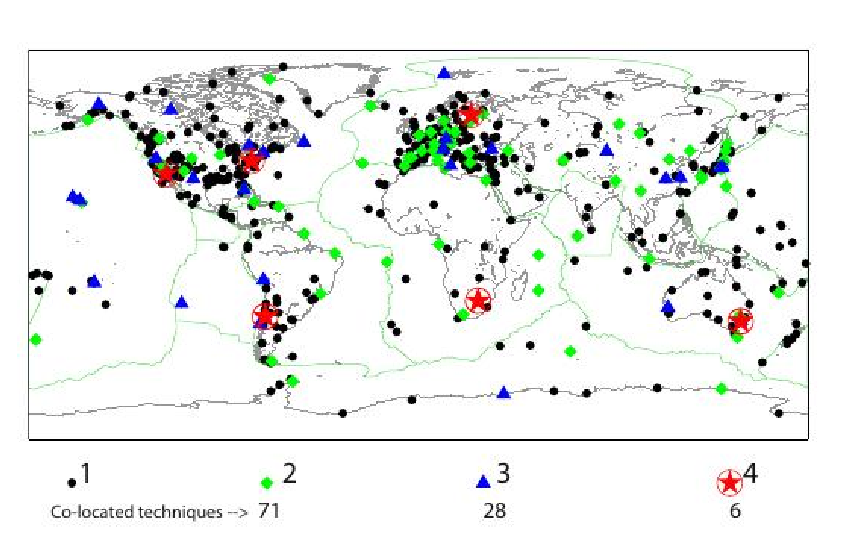
\includegraphics[scale=0.7]{ch2_ITRF_2008.eps}
\caption{\textit{Sieć stacji referencyjnych tworząca układ ITRF2008} źródło: \cite[][strona 38]{IERS_2010}}
\label{fig:ch2_itrf_2008}
\end{figure}
Układ ITRF składa się ze współrzędnych oraz prędkości wybranych stacji referencyjnych oraz ich macierzy kowariancji. Parametry te są wyznaczane 
w centrach obliczeniowych Międzynarodowej Służby Ruchu Obrotowego Ziemi oraz Systemów Odniesienia (IERS) i publikowane w IERS Conventions \cite[][strona 167]{ROCZNIK_2014}.
Warto jeszcze raz podkreślić, że dokładność wszystkich produktów służby IGS (International GNSS Service) takich jak orbity satelitów jest determinowana 
przez dokładność układu odniesienia do jakiego są one transformowane ( z układu niebieskiego ICRF) i następnie publikowane. Dokładność produktów IGS 
ma bezpośredni wpływ na wynik rozwiązania pozycji podczas nawigacji w czasie rzeczywistym.
Układ odniesienia IGS jest determinowany na podstawie tylko obserwacji GNSS wykonywanych na starannie wyselekcjonowanym podzbiorze 
stacjach referencyjnych IERS, i wpasowywany następnie za pomocą 14 parametrowej transformacji Helmerta do układu ITRF2008 \cite[]{ALTAMIMI_2009}.
Globalny układ odniesienia IGS jest zatem zgodny z układem ITRF2008. Ponadto wszystkie dane powstałe przed rokiem 2008 zostały odpowiednio 
przetransformowane w celu osiągnięcia jak największej wewnętrznej spójności \cite[][strona 15]{KOUBA_2009}.
Dla lepszego zrozumienia dalszych rozdziałów kluczowe wydaje się wyjaśnienie, że współrzędne stacji referencyjnych w układzie ITRF 
są wolne od wpływu pływów oceanicznych, pływów skorupy ziemskiej, oraz zmian położenia osi obrotu Ziemi (tzw. ruch bieguna).
W sensie globalnym pozycja każdej stacji referencyjnej podlega periodycznym fluktuacjom, których amplituda jest rzędu kilku
decymetrów. W układzie ITRF powyższe wysokie częstotliwości są eliminowane za pomocą zastosowanych modeli. W pomiarach względnych o krótkich
bazach (<100km) fluktuacje są w przybliżeniu takie same, zatem do współrzędnych ITRF nie jest konieczne wprowadzanie poprawek.
Poprawki są jednak konieczne gdy wykonujemy pomiary w sensie absolutnym (aktualną pozycję wyznaczamy bezpośrednio względem znanych orbit)
w technice PPP, lub w przypadku gdy pomiary różnicowe wykonywane są dla dużych odległości. \cite[][strona 11]{KOUBA_2009}

\section{Globalne Systemy Nawigacji Satelitarnej GNSS}
\noindent Znaczenie akronimu GNSS (Global Navigation Satellite Systems) nie jest jednoznaczne. Większość środowiska naukowego 
postrzega ostatni wyraz skrótu w liczbie mnogiej - systemy, takiej też interpretacji przyjęto używać w niniejszej pracy.
Dzieje się tak ponieważ, jest kilka systemów satelitarnego pozycjonowania. Większość z nich 
została opisana pokrótce w dalszej częsći tego podrozdziału. Jednakże, jeżeli spojrzymy na systemy GNSS z punktu widzenia rozwiązania 
nawigacyjnego bazującego na sygnałach pochodzących od różnych satelitów ( w sensie przynależności do konkretnego systemu), wtedy jako całość 
tworzą one jeden globalny system nawigacji satelitarnej \cite[][strona vii]{hofmann_gnss}.\\
\indent Systemy GNSS są sukcesorami systemów dopplerowskich - systemu Transit\footnote{Pierwszy
działający system nawigacji satelitarnej, używany przez marynarkę wojenną USA 
do określania pozycji okrętów podwodnych z dokładnością 25m. Działanie oparte na efekcie Dopplera.} oraz Cikada\footnote{Stworzony przez naukowców byłego ZSRR 
jako odpowiednik systemu Transit}, Bazują na od około 30 do 45 satelitów umieszczonych na tzw. średnich orbitach MEO\footnote{MEO 
(Medium Earth Orbit) - średnia orbita okołoziemska w której wysokość satelity względem Ziemi waha się od 2000km do 35786km - wysokość orbity geostacjonarnego)}
oraz emitujących fale radiowe w zakresie mikrofalowym na dwóch lub więcej częstotliwościach.
Pasmo mikrofalowe pozwala na używanie systemów niezależnie od panujących warunków pogodowych, natomiast sygnał emitowany na przynajmniej dwóch częstotliwosciach 
pozwala na eliminację negatywnego wpływu refrakcji jonosferycznej \cite[][strona 33]{ggos}. Quasi-symultaniczna obserwacja przez odbiornik kilku różnych 
satelitów GNSS eliminuje w znacznym stopniu błąd zegara odbiornika. Wszystkie systemy GNSS są pasywne - odbiornik nie musi wysyłać żadnych sygnałów do satelitów w 
celu wykonania pomiaru. Opisane właściwości uczyniły systemy GNSS niejako \enquote{koniami pociągowymi} nawigacji oraz geodezji kosmicznej \cite[][strona 36]{ggos}.\\
\indent W każdym systemie GNSS wyróżnić można trzy główne części: segment kosmiczny, segment użytkowników oraz segment kontrolny.
Zadaniem segmentu kosmicznego jest zapewnienie takiej konstelacji satelitów, która pozwoli na określanie pozycji oraz prędkości
użytkownika niezależnie od jego połorzenia na Ziemi.
Segment kontrolny steruje całym systemem poprzez uaktualnianie danych komputerów pokładowych satelitów oraz ochroną systemu przed nieautoryzowanymi użytkownikami.\\
\indent Należy dodać, że istanieje cały szereg systemów wspomagania GNSS w zastosowaniach nawigacyjnych, które podobnie dzielimy na kosmiczne - SBAS\footnote{
SBAS - space based augmentation systems} oraz naziemne - GBAS\footnote{GBAS - ground based augmentation systems}.
Kosmiczne systemy wspomagania składają się z sieci naziemnych stacji referencyjnych generujących poprawki różnicowe oraz informacje o sprawności systemu GNSS, 
które są dystrybuowane za momocą satelitów geostacjonarnych. W systemach GBAS odbiorniki referencyjne montowane są jedynie w pobliżu lotnisk, a poprawki 
transmitowane są drogą radiową. Przykładami SBAS są Europejski system EGNOS\footnote{EGNOS - European Geostationary Navigation Overlay Service.} 
oraz system WAAS\footnote{Wide Area Augmentation System} obejmujący swoim zasięgiem Amerykę Północną. 
	\subsection{GPS}
\noindent System GPS został stworzony przez Departament Obrony USA z myślą o wyznaczaniu pozycji, prędkości oraz synchronizacji czasu obiektów wojskowych
w globalnym układzie odniesienia, niezależnie od warunków pogodowych oraz lokalizacji użytkownika na Ziemi \cite[][strona 309]{hofmann_gnss}.
System GPS zarządzany przez Siły Powietrzne USA, osiągnął pełną operacyjność 17 lipca 1995r. System składa się z segmantu kosmicznego, kontrolnego oraz z segmantu użytkowników.
Segmant kosmiczny tworzy konstelacja satelitów GPS transmitujących sygnały radiowe do użytkowników. Rząd Stanów Zjednoczonych zobowiązał się do 
utrzymywania w przestrzeni kosmicznej minimum 24 satelity w ciągu 95\% czasu. Obecnie w przestrzeni znajduje się 31 satelitów krążących wokół Ziemi na 
wysokości około 20200km, z których wyróżniamy 27 satelitów bazowych czynnych, w załorzeniu nieprzerwanie. 
Każdy obiega naszą planetę dwókrotnie w ciągu doby, poruszając się na jednej z sześciu orbit kołowych rozmieszczonych równomiernie co 60\degree,
nachylonych względem płaszczyzny równika pod kątem 55\degree \cite[]{GPS_GOV}. Poniżej na rysunku \ref{fig:gps_space_segment} przedstawiono operacyjne satelity systemu GPS
bloku II.
\begin{figure}[H]
\centering
\begin{subfigure}{.2\textwidth}
  \centering
  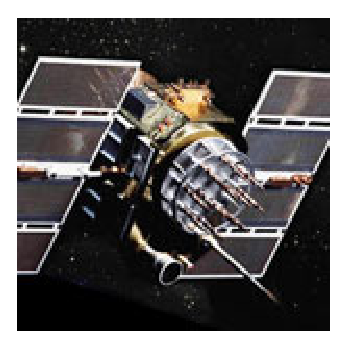
\includegraphics[width=.9\linewidth]{chapter2_gps_space_1.eps}
  \caption{blok IIa}
  \label{fig:block2a}
\end{subfigure}%
\begin{subfigure}{.2\textwidth}
  \centering
  
\includegraphics[width=.9\linewidth]{chapter2_gps_space_2.eps}
  \caption{blok IIR}
  \label{fig:block2r}
\end{subfigure}
\begin{subfigure}{.2\textwidth}
        \centering
        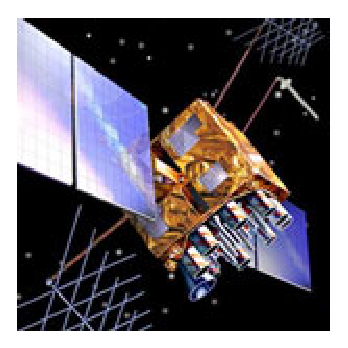
\includegraphics[width=.9\linewidth]{chapter2_gps_space_3.eps}
        \caption{blok IIR(M)}
        \label{fig:block2rm}
\end{subfigure}
\begin{subfigure}{.2\textwidth}
        \centering
        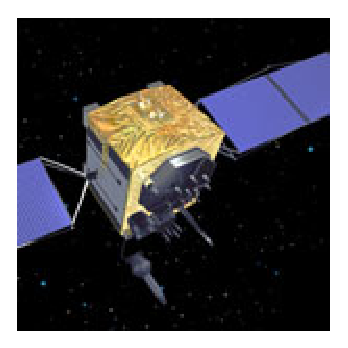
\includegraphics[width=.9\linewidth]{chapter2_gps_space_4.eps}
        \caption{blok IIF}
        \label{fig:block2f}
\end{subfigure}
\caption{\textit{Operacyjne satelity systemu GPS}
źródło: \cite[]{GPS_GOV}}
\label{fig:gps_space_segment}
\end{figure}
\indent Segment kontrolny systemu GPS składa się z sieci stacji przedstawionych na rysunku \ref{fig:gps_control_segment} ze stacją główną zlokalizowaną w stanie Colorado.
Zadaniem stacji kontrolnych jest śledzenie satelitów systemu GPS, kontrolowanie jakości transmisji danych, uaktualnianie danych oraz komputerów pokładowych znajdujących się
na satelitach oraz sterowanie konstelacją GPS. Ze względu na załorzenia niniejszej pracy segment użytkowników został zawężony głównie do rolnictwa precyzyjnego i traktuje o
nim niejako cała praca.
\begin{figure}[H]
\centering
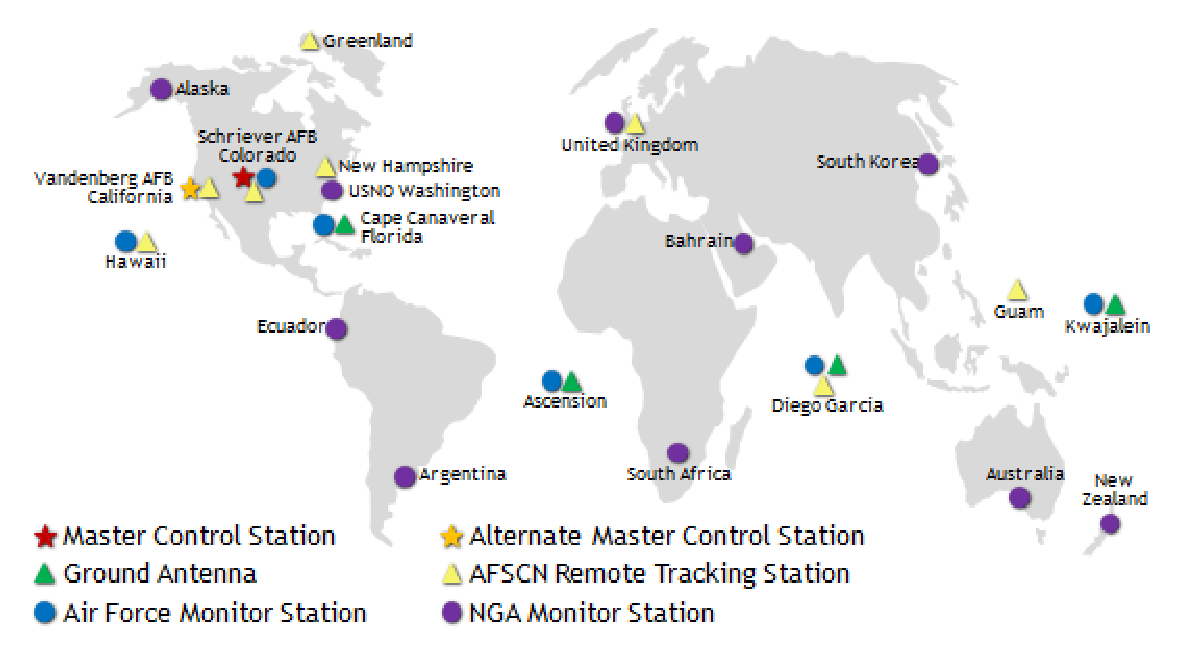
\includegraphics[scale=0.5]{chapter2_control_segment.eps}
\caption{\textit{Stacje segmentu kontrolnego GPS} źródło: \cite[]{GPS_GOV}}
\label{fig:gps_control_segment}
\end{figure}
\indent Sygnały wysyłane przez satelity dzielą się na militarne oraz do zastosowań cywilnych. Sygnały militarne są kodowane, zatem w niniejszej pracy pokrótce opisano
tylko sygnały ogólnodostępne. Satelity GPS emitują fale elektromagnetyczne w paśmie radiowym. Wyróżniamy trzy częstotliwości nośne dla sygnałów GPS: 
L1 - częstotliwość podstawowa, L2 - Początkowo tylko do zastosowań wojskowych, od 2005 roku jest dostępna do zastosowań cywilnych, L5 - od kwietnia 2014r. pojawiła się 
depesza nawigacyjna dostępna użytkownikom cywilnym. Częstotliwość L5 znajduje się w paśmie radiowym zarezerwowanym dla branży lotniczej \cite[]{GPS_GOV}.
Rysunek \ref{fig:gps_freequencies} przedstawia tabelę częstotliwości nośnych GPS.
\begin{figure}[H]
\centering
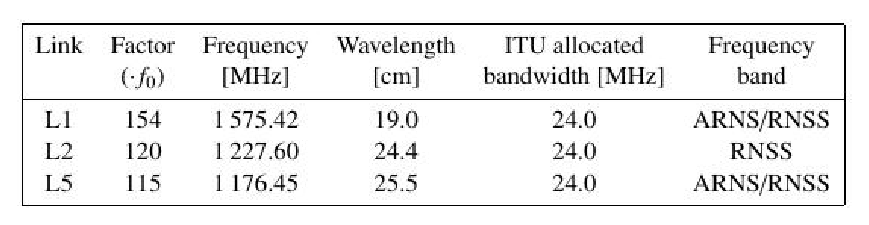
\includegraphics[scale=0.9]{chapter2_gps_freequencies.eps}
\caption{\textit{Częstotliwości nośne sygnału GPS} źródło: \cite[][strona 329]{hofmann_gnss}}
\label{fig:gps_freequencies}
\end{figure}
\noindent Bazując na powyższych częstotliwościach generowane są dane nawigacyjne w postaci tzw. kodów na których opierają się algorytmy wyznaczania pozycji odbiornika.
C/A jest kodem propagowanym na częstotliwości L1 wraz z depeszą nawigacyjną, przeznaczonym dla użytkoników cywilnych do wyznaczania pozycji w czasie rzeczywistym.
C/A jest kodem stosunkowo krótkim (297m), co pozwala na bardzo szybką inicjalizację,
lecz co za tym idzie sygnał jest bardzo łatwo podatny interferencje \cite[][strona 332]{hofmann_gnss}.
P(Y) - kod którego długość wynosi około 266.4 dni ze względu na tę właśnie cechę charakteryzuje się niemożnością jego odbierania bez apriorycznej znajomości dokładnej 
poprawki zegara, pozycji oraz efemeryd satelitów. Modulowany na dwóch częstotliwościach L1 oraz L2 kod P(Y) w zastosowaniach nawigacyjnych jest przeznaczony jedynie dla wojska.
Kodem, który jest modulowany na częstotliwości nośnej L2 i przeznaczonym do zastosowań komercyjnych jest kod L2C. Kod L2C poprzez kombinacje liniowe z kodem C/A pozwala 
na korekcję negatywnego wpływu jonosfery. Użytkownicy cywilni którzy dysponują dwuczęstotliwościowymi odbiornikami dzięki kodowi L2C są w stanie uzyskać porównywalną
dokładność jaką uzyskują użytkownicy autoryzowani na kodzie P(Y). L2C pozwala na szybszą inicjalizację odbiornika, podnosi niezawodność oraz niejako dostępność sygnału 
GPS poprzez transmisję z wyższą efektywną mocą sygnału \cite[]{GPS_GOV}. Kolejnym kodem jest L5C. Kod L5C modulowany na częstotliwośći L5 został specjalnie zaprojektowany 
aby sprostać wymaganiom aplikacji służących do celów zapewniania bezpieczeństwa życia ludzkiego \cite[][strona 335]{hofmann_gnss}. Kod L5C charakteryzuje się wysoką mocą 
sygnału oraz przepustowością danych. L5C w kombinacji z kodem C/A zwiększy istotnie dokładność poprzez eliminację wpływy jonosfery. Sygnał na częstotliwości L5 
począwszy od 31 grudnia 2014 jest już eksperymentalnie dostępny dla użytkowników. Możliwe jest już zatem wykonywanie obserwacji sygnału GPS na trzech częstotliwościach nośnych,
co prawdopodobnie pozwoli na uzyskanie sub-metrowych dokładności bez użycia wsparcia systemów augmentacyjnych \cite[]{GPS_GOV}. W planach modernizacyjnych systemu GPS jest,
także wprowadzenie dodatkowego (oprócz C/A) kodu na częstotliwości L1 - L1C. Wprowadzenie jeszcze jednego kodu na częstotliwości L1 pozwoli na ulepszenie pozycji 
odbiorników mobilnych w miastach bądź w innych trudnych terenach. Ponadto warto zwrócić uwagę na fakt, że kod L1C został zaprojektowany wspólnie przez Europę oraz 
Stany Zjednoczone jako wspólny sygnał zarówno dla GPS jak i Galileo. Kod L1C docelowo ma być emitowany przez wszystkie dostępne systemy satelitarne \cite[]{GPS_GOV}.\\
\indent Układ odniesienia względem, którego jest wyznaczana pozycja GPS to układ WGS84\footnote{WGS84 (World Geodetic System) geocentryczny ortokartezjański układ współrzędnych
zbudowany pocztkowo w oparciu o obserwacje satelitów systemu Transit. Wraz z rozwojem technologii GPS układ został zmodernizowany czterokrotnie.
Obecna realizacja to układ WGS84(1674) z lutego 2012 roku. Obecnie układ WGS84 jest zarządzany przez jedną z agencji wywiadu USA - National Geospatial Intelligance Agency.}
,zdefiniowany poprzez wyznaczenie współrzędnych oraz prędkości stacji referencyjnych jako realizacja systemu WGS84. Współrzędne stacji referencyjnych są następnie 
używane do wyznaczanie orbit satelitów GPS. Dokładność układu WGS84 względem aktualnego układu Ziemskiego ITRF jest centymetrowa \cite[][strona 51]{donnelly}.
Należy zauważyć, że w zależności od kontekstu WGS84 odnosi się do systemu, układu odniesienia lub referencyjnej elipsoidy.
Centymetrowa dokładność aktualnej realizacji układu odniesienia systemu GPS względem układu ITRF2008 na epokę 2005
wynika bezpośrednio ze zgodności na poziomie definicyjnym systemów WGS84 oraz ITRS. Drobne różnice wynikają z tego, że do realizacji systemu WGS84 w celu uzyskania jak 
największej spójniości danych używane są jedynie obserwacje GPS. Elipsoida\footnote{Powierzchnia powstała poprzez obrót elipsy o zadanych parametrach wokół jej 
krótszej półosi. W tym konkretnym przypadku środek elipsoidy jest umieszczony w środku masy Ziemi, a jej krótsza półoś pokrywa się z osią Z układu odniesienia WGS84.}
WGS84 jest powierzchnią odniesienia aproksymującą kształt oraz rozmiary Ziemi. Różnica między elipsoidą GRS80 złączoną z układem ITRF a elipsoidą WGS84 jest z punktu 
widzenia dokładności wyznaczeń na potrzeby nawigacji zaniedbywalna \cite[][strona 50]{donnelly}.\\
\indent System czasu Systemu GPS jest oparty o wzorzec czasu atomowego. Nominalnie czas GPS różni się od Międzynarodowego Czasu Atomowego TAI o 19 sekund, i jest 
ścisle związany z Uniwersalnym Czasem Koordynowanym UTC.\\
Podsumowując ten paragraf można powiedzieć, że system GPS już od ponad dwóch dekad jest nieocenionym, dla takich dziedzin działalności człowieka jak:
Budownictwo, Energetyka, Geodezja z Geodynamiką, Przemysł wydobywczy, Transport, Ratownictwo, Rolnictwo oraz wiele innych.
 	\subsection{GLONASS}
Podobnie jak system GPS powstał na podstawie doświadczeń z systemem Transit, tak system GLONASS został zbudowany z doświadczeń sowieckich naukowców 
z systemem Cikada. GLONASS jest systemem wojskowym, i podobnie jak GPS zaprojektowanym do dostarczania nielimitowanej liczbie użytkowników, niezależnie od pogody,
trójwymiarowej pozycji, synchronizacji czasu, oraz prędkości w obrębie całego globu \cite[][strona 342]{hofmann_gnss}. Operacyjność systemu ogłoszono w 1993r. 
jednakże nominalną konstelację 24 satelitów system osiągnął dopiero 18 stycznia 1996r. Z powodu kryzysu ekonomicznego Federacji Rosyjskiej liczba operacyjnych 
satelitów systematycznie spadała i w roku 2001 osiągnęła minimum w postaci liczby sprawnych satelitów poniżej dzsiesięciu \cite[][strona 342]{hofmann_gnss}.
Do pełnej operacyjności system GLONASS powrócił po około 10 latach 8 grudnia 2011 roku \cite[]{glonass_geoforum}.\\
\indent Segment kosmiczny systemu GLONASS składa się z 24 satelitów poruszających się na orbitach kołowych na wysokości około 19100km nad powierzchnią Ziemi.
Okres obiegu wokół Ziemi satelitów systemu GLONASS wynosi 11 godzin 15 minut i 44 sekundy. Konstelacja satelitów jest zgrupowana w trzech płaszczyznach o inklinacji\footnote{
Inklinacja w tym kontekście określa kąt dwuścienny między płaszczyzną orbity satelity a płaszczyzną równika.} równej 64.8\degree - w każdej znajdują się 
orbity ośmiu satelitów równomiernie rozmieszczonych (co 45\degree). Węzły wstępujące orbit satelitów należących do różnych płaszczyzn różnią się o 120\degree.
Opisana konstelacja pozwala na symultaniczną widoczność minimum pięciu satelitów z około 99\% powierzchni Ziemi \cite[][strona 349]{hofmann_gnss}.\\
\indent Segment kontrolny systemu GLONASS dzieli się na \begin{inparaenum}[1)] \item centrum sterowania systemem 
\item stacje śledzące \end{inparaenum}. Centrum sterowania systemem dzieli się na centralny moduł sychronizacyjny (Schelkowo w regionie moskiewskim) odpowiedzialny
za synchronizację czasu systemu GLONASS oraz część kontrolną (Krasnoznamensk 70km od Moskwy) gdzie ma miejsce zarządzanie wszystkimi funkcjami systemu oraz planowanie.
Stacje śledzące są podzielone na trzy grupy: \begin{inparaenum}[a)] \item cztery stacje TT\&C wspomagane pięcioma stacjami pomiarów laserowych służące do
śledzenia i monitorowania satelitów oraz wysyłania do nich wiadomości. \item cztery stacje służące do kontroli urządzeń elektronicznych. 
\item stacje optyki kwantowej \end{inparaenum}. Niestety znacząca część informacji dotyczących segmentu kontrolnego systemu GLONASS
nie jest dostępna publicznie \cite[][strona 353]{hofmann_gnss}.\\
\indent Czas systemu GLONASS jest zarządzany przez wspomniany powyżej moduł synchronizacyjny za pomocą maserów wodorowych. Czas ten jest ściśle powiązany z czasem uniwersalnym 
koordynowanym. Stałe przesunięcie wynoszące plus trzy godziny związane jest różnicą między czasem Moskiewskim oraz Greenwich. Ponadto występuje losowa 
rozbierzność nieprzekraczająca 1ms, która wynika z tego, iż wspomniane skale czasu są utrzymywane przez różne zegary \cite[][strona 346]{hofmann_gnss}.\\
\indent Jako system odniesienia systemu GLONASS oryginalnie przyjęto sowiecki SGS-85, który zamieniono w roku 1990 na SGS-90\footnote{ SGS (Soviet Geodetic System) Sowiecki 
System Odniesień Przestrzennych}. Realizacja systemu to Kartezjański układ współrzędnych otrogonalnych PE-90 zrealizowany poprzez określenie współrzędnych 26 stacji 
refrencyjnych. Różnica układu PE-90 względem układu ITRF jest dość znaczna jeżeli chodzi o wymagania dokładnościowe rolnictwa precyzyjnego.
Dla przykładu wielka półoś elipsoidy geocentrycznej PE-90 jest aż o metr krótsza od odpowiadającego parametru elipsoidy GRS80. Należy jednak zaznaczyć, że 
różnice współrzędnych punktów nie przekraczają 15 metrów (średnio 5m).
Współrzędne z układu PE-90 do układu ITRF transformuje się za pomocą transformacji siedmioparametrowej wyznaczanej za
pomocą porównania tras satelitów glonas dostępnych w obu układach odniesienia \cite[]{WGS84_PZ90}.\\
\indent System GLONASS podobnie jak system GPS dostarcza wysokiej jakości sygnałów dla użytkowników autoryzowanych, oraz standardowej dokładności sygnału 
dla użytkowników cywilnych. Obecnie sygnały satelitarne systemu są przenoszone za pomocą dwóch pasm częstotliwości fali radiowej: G1 = 1602Mhz oraz G2 = 1246Mhz.
W planowanej trzeciej generacji system będzie emitował dodatkowy sygnał modulowany w paśmie częstotliwości G3 = 1204.704Mhz w podobieństwie do trzeciej częstotliwości L5 
systemu GPS. Tym co diametralnie różni system GLONASS od systemu GPS jest to, że każdy satelita moduluje swój sygnał na fali radiowej o unikalnej dla niego częstotliwości.
Na rysunku \ref{fig:glonas_freq} przedstawiona została tabela według której każdemu satelicie przyporządkowywana jest unikalna częstotliwość.
\begin{figure}[H]
\centering
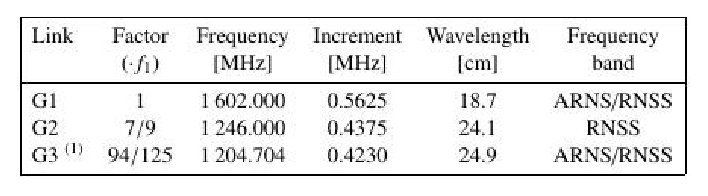
\includegraphics[scale=1.1]{chapter2_glonass_freq.eps}
\caption{\textit{Częstotliwości nośne sygnału GLONASS} źródło: \cite[][strona 357]{hofmann_gnss}}
\label{fig:glonas_freq}
\end{figure}
Tak samo jak w systemie GPS odpowiednik kodu C/A jest modulowany w paśmie częstotliwości G1 i jest nośnikiem standardowej usługi pozycjonowania.
Wysokiej dokładności sygnał P nie jset kodowany (w przeciwieństwie do GPS) i jest modulowany na obu falach nośnych G1 oraz G2. Począwszy od roku 2004 
kod standardowej dokładności jest także dostępny w paśmie G2. Na koniec warto odnotować, że pod pewnymi względami zastosowane w systemie GLONASS rozwiązania 
są lepsze niż te z systemu GPS. Większa inklinacja orbit pozwala średnio obserwować więcej satelitów, a unikalne częstotliwości sygnału dla każdego satelity 
znacząco zmniejszają niekorzystne efekty interferencji \cite[][strona 355]{hofmann_gnss}.
	\subsection{GALILEO}
System GALILEO zaprojektowano głównie na potrzeby Unii Europejskiej w celu ekonomicznego oraz strategicznego uniezależnienia jej od systemu GPS.
Ze względu na to, że system GALILEO nie jest jeszcze operacyjny (aktualnie 8 satelitów), w pracy postanowiono opisać tylko jego najważniejsze załorzenia projektowe.\\
\indent Segment kosmiczny systemu GALILEO docelowo ma się składać z 30 satelitów (27 + 3 zapasowe) po 9 satelitów operacyjnych na jedną płaszczyznę orbitalną.
Inklinacje płaszczyzn mają wynosić 56\degree. Satelity będą się poruszały po orbitach prawie kołowych na wysokości 23616km równomiernie rozmieszczone co 40\degree w 
płaszczyźnie orbity. Tak zaprojektowana konstelacja zapewnić ma globalną widoczność minimum 6 satelitów na wysokości powyżej 10\degree nad horyzontem.\\
\indent Segmant naziemny systemu GALILEO został zaprojektowany tak aby składał się z części kontrolnej stanu technicznego konstelacji satelitów oraz 
części operacyjnej, która ma odpowiadać za całościowe funkcjonowanie systemu (depesze satelitów, kontrola danych, kontrola czasu oraz wiele innych). Warto nadmienić,
że wśród stacji segmentu naziemnego oprócz klasycznej infrastruktury śledzącej satelity (kilkuczęstotliwościowe odbiorniki) znajdą się także stacje pomiarów laserowych.
\cite[][strona 380]{hofmann_gnss}. Ponadto zaprojektowano także budowę lokalnych stacji obserwacyjnych kontrolujących niezawodność systemu.\\
\indent System GALILEO ma być oparty na geocentrycznym układzie odniesienia GTRF\footnote{Galileo Terrestial Reference Frame}, który będzie powiązany z ITRF.
Z załorzeń projektowych wynika, że różnica pomiędzy GTRF oraz ITRF nie może przekraczać trzech centymetrów na poziomie ufności 2$\sigma$.\\
\indent Czas systemu GALILEO GST\footnote{Galileo System Time} będzie oparty na ciągłej skali czasu atomowego, zsynchronizowanej z Międzynarodowym Czasem Atomowym TAI i
podtrzymywanej za pomocą maserów wodorowych. System czasu GALILEO będzie używał korekt czasu pochodzących od zewnętrznych ośrodków takich jak Międzynarodowe 
Biuro Miar i Wag w celu bezpośredniej synchronizacji z UTC. Maksymalna rónica midzy GST a czasem atomowym TAI ma nie przekraczać 50ns na poziomie ufności 95\%.\\
\indent Podczas projektowania systemu GALILEO przyjęto podejście nastawione na serwisy jakich system ma dostarczać użytkownikom.
Adekwatnie do potencjalnego zapotrzebowania na usługi wyróżniono następujące grupy:
\begin{itemize}
\item Serwis otwarty (OS) - dostępny dla wszystkich użytkowników bezpłatnie. Charakteryzuje się brakiem informacji na temat wiarygodności systemu.
Przeznaczony jest do uzyskiwania pozycji oraz referencji czasowej nie wymagających wysokiej dokładności. Sześć jawnych kodów jest modulowanych na fale radiowe o 
trzech częstotliwościach nośnych. Jednoczęstotliwościowe odbiorniki systemu GALILEO będą wyznaczać pozycję porównywalną z rozwiązaniem opartym o kod C/A GPS.
\item Serwis komercyjny (CS) - różniący się od serwisu otwartego gwarancją dostępności oraz dostępem do dodatkowych szyfrowanych danych zawartych w depeszy nawigacyjnej 
propagowanej za pomocą modulacji sygnału na trzech częstotliwościach nośnych. 
\item Serwis bezpieczeństwa życia (SoL) - bazuje na tych samych sygnałach co serwis otwarty. W tym trybie w depeszy nawigacyjnej zawarta będzie informacja o wiarygodności 
systemu GALILEO. Jakiekolwiek awarie będą sygnalizowane odpowienimi ostrzeżeniami wysyłanymi do użytkownika.
\item Serwis publiczny regulowany (PRS) - przeznaczony dla służb, agencji rządowych bądź innych podmiotów zajmujących się ochroną obywateli, obronnością oraz dbaniem o
respektowanie prawa. Głównym celem serwisu jest dostarczanie silnego ciągłego oraz zakodowanego sygnału, który będzie możliwy do użycia nawet w sytuacjach kryzysowych.
Sygnał w tym serwisie będzie modulowany na dwie częstotliwości nośne aby zmaksymalizować odporność na interferencje, przy jednoczesnej minimalizacji ryzyka celowych
zakłóceń zewnętrznych. W serwisie tym będzie również dostępna informacja o wiarygodności systemu GALILEO.
\item Serwis ratunkowy (SAR) - Serwis polage na wykrywaniu przez satelity systemu sygnałów ratunkowych (406Mhz), a następnie na przesyłaniu tej informacji do 
centrum segmentu naziemnego, które ma za zadanie powiadomić odpowiednie służby.
\end{itemize}
\indent System GALILEO ma wykorzystywać trzy pasma częstotliwości fali radiowych L1, E5, E6 na, których będzie możliwa modulacja dziesięciu różnych sygnałów.
Rysunek \ref{fig:galileo_freq} przedstawia schemat przydziału częstotliwości nośnych poszczególnym sygnałom systemu GALILEO.
Trzy sygnałý nawigacyjne modulowane na częstotliwości E1: Dwa nieszyfrowane sygnały E1B orax E1C dostępne dla wszystkich użytkowników. E1B oprócz wiadomości nawigacyjnej 
przenosić ma szyfrowane dane komercyjne oraz informacje o wiarygodności. Kanał danych E1B oraz kanał pilotażowy E1C mają wspierać usługi: otwartą, komercyjną oraz 
usługę ratowania życia. Zaszyfrowany komponent E1A ma być dostępny tylko dla autoryzowanych użytkowników w serwisie (PRS) \cite[][strona 387]{hofmann_gnss}.
Podobnie do pasma częstotliwości E1, pasmo E6 również ma być nośnikiem trzech sygnałów: E6A, E6B, E6C dostępnych komercyjnie. 
Sygnał E6B ma być nosnikiem depeszy nawigacyjnej oraz szyfrowanych danych komercyjnych. Sygnał E6C ma być kanałem pilotażowym a E6A wspierać serwis regulowany (PRS)
\cite[][strona 389]{hofmann_gnss}.
Pasmo częstotliwości E5 jest nośnikiem czterech sygnałów. W pasmach E5a oraz E5b przenoszone są dwie pary: kanał danych plus kanał pilotażowy.
\begin{figure}[H]
\centering
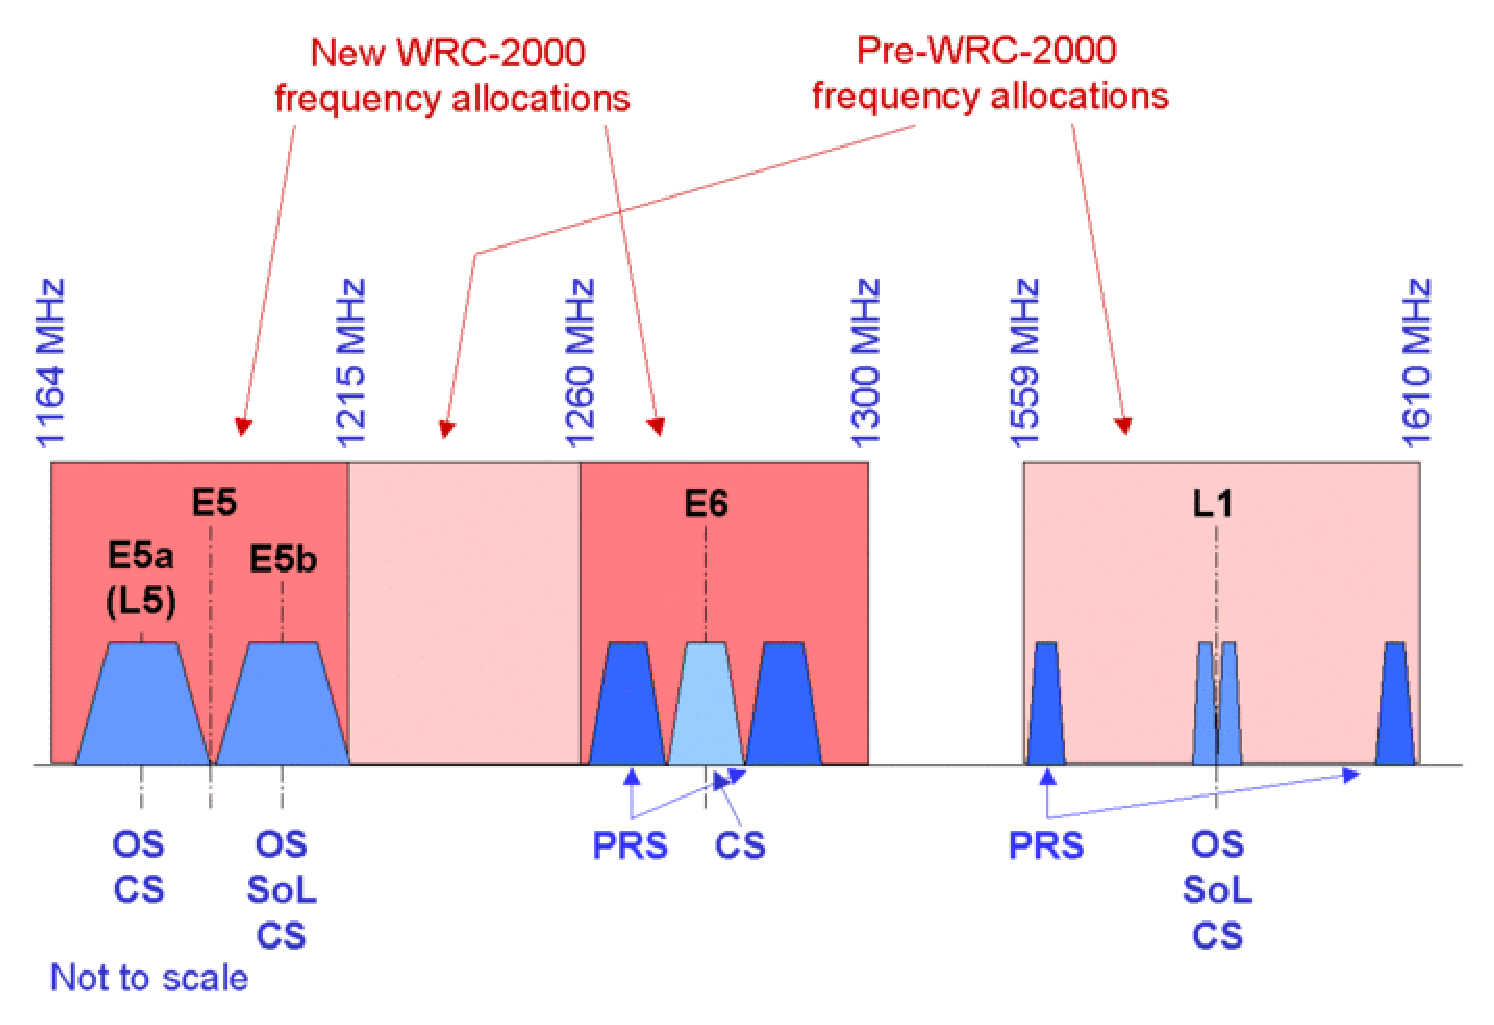
\includegraphics[scale=0.6]{chapter2_galileo_freq.eps}
\caption{\textit{Schemat częstotliwości nośnych sygnałów systemu GALILEO} źródło: \protect\url{http://www.esa.int/spaceinimages/Images/2005/04/Galileo_signal_frequencies}}
\label{fig:galileo_freq}
\end{figure}
\section{Algorytmy Pozycjonowania}
Algorytmy pozycjonowania w nawigacji satelitarnej opierają się głównie na dwóch typach obserwacji: 
\begin{itemize}
	\item pomiarze czasu propagacji sygnału od satelity do odbiornika - obserwacje kodowe
	\item obserwacje fazowe - obliczane jako różnice fazy fali radiowej docierającej od satelity do odbiornika oraz fazy sygnału referencyjnego 
	generowanego w odbiorniku (chwilowa faza wypadkowego sygnału). Od momentu (epoka $t_0$) rozpoczęcia śledzenia sygnału wypadkowego o tzw. częstotliwości dudnienia,
	zliczana jest również przez odbiornik całkowita liczba jego pełnych cykli fazowych.
\end{itemize}
\indent Równanie obserwacji kodowych tzw. równanie psełdoodległości oparte jest na różnicy momentów czasu emisji $t^s$ oraz odbioru $t_r$ sygnału, pomnożonej 
przez prędkość światła $c$ \cite[][strona 11]{BOSY_2005}. Wyraża się następującą zależnością (na podstawie \cite[]{BOSY_2005}):
\begin{equation}
	R_r^s = (t_r - t^s)c = \rho_r^s + c({\delta}t_r - {\delta}t^s) + {\delta}T_r^s + {\delta}I_r^s + {\delta}_r^s + \epsilon
	\label{eq:code_general}
\end{equation}
Gdzie:
$t^s$, $t_r$ - oznaczają odpowiednio momenty wysłania i odbioru sygnału GNSS $\big[s\big]$,\newline
${\delta}t^s$, ${\delta}t_r$ - oznaczaja odpowiednio błąd zegara satelity i odbiornika $\big[s\big]$,\newline
$c$ - prędkość światła w próżni równą 299 792 458 $\big[\frac{m}{s}\big]$,\newline
$\rho_r^s$ - stanowi odległość geometryczną między satelitą a odbiornikiem $\big[m\big]$,\newline
${\delta}T_r^s$ - opóźnienie spowodowane refrakcją troposferyczną $\big[m\big]$,\newline
${\delta}I_r^s$ - opóźnienie spowodowane refrakcją jonosferyczną $\big[m\big]$,\newline
${\delta}_r^s$ - czynnik reprezentujący błędy systematyczne satelity i odbiornika $\big[m\big]$,\newline
$\epsilon$ - stanowi błędy przypadkowe o rozkładzie normalnym $\big[m\big]$,\newline
W równaniu \ref{eq:code_general} występują cztery niewiadome: ${\delta}t_r$ - błąd zegara odbiornika oraz występujące w równaniu odległości geometrycznej\footnote{
${\rho}_r^s = \sqrt[2]{{\big(X^s - X_r\big)}^2 + {\big(Y^s - Y_r\big)}^2 + {\big(Z^s - Z_r\big)}^2}$}
współrzędne odbiornika $\big(X_r, Y_r, Z_r\big)$. Dlatego do określenia pozycji potrzebne jest wykonanie symultanicznie obserwacji do 
minimum czterech satelitów. Współrzędne satelity $\big(X^s, Y^s, Z^s\big)$ na epokę $t^s$ oraz błąd jej zegara ${\delta}t^s$ są w 
przybliżeniu określane na podstawie danych znajdujących się w depeszy nawigacyjnej \cite[][strona 11]{BOSY_2005}.
Źródła błędów spowodowane propagacją sygnału w atmosferze (${\delta}T_r^s$, ${\delta}I_r^s$), błędy systematyczne oraz sposoby ich eliminacji 
zostaną omówione i porównane wspólnie dla obserwacji kodowych oraz fazowych w dalszej części tego podrozdziału. Warto jedynie zaznaczyć, że wpływ jonosfery\footnote{
Jonosfera w przybliżeniu obejmuje warstwy atmosfery znajdujące się między wysokościami $h_1 = 50km$ oraz $h_2 = 1000km$. Jest ośrodkiem dyspersyjnym (propagacja 
fali zależy od jej częstotliwości) w stosunku do sygnałów radiowych GNSS.} 
na obserwacje kodowe powoduje zmniejszenie szybkości grupowej propagacji fali elektromagnetycznej $v_{gr}$ (rozumianej jako prędkość rozchodzenia się czoła fali), a 
w związku z tym mierzone psełdoodległości obarczone jej wpływem są zawsze zbyt długie. Wpływ troposfery również powoduje nadmiarowość w zmierzonej psełdoodległości.  
Określanie pozycji anteny odbiornika na podstawie obserwacji kodowych stanowi podstawę rozwiązań nie wymagających dużej dokładności.\newline
\indent W pracy \cite[]{hofmann_gnss} profesor Bernard Hofmann opisał szczegółowo zasadę pomiarów fazowych, włącznie z wyprowadzeniem równania tychże obserwacji.
Przy załorzeniu zaniedbywalnych odchyleń częstotliwości sygnałów satelity oraz odbiornika od częstotliwości nominalnej,
faza sygnału referencyjnego generowanego przez odbiornik wyraża się równaniem \ref{eq:generated_phase},
a faza sygnału odebranego od satelity i zrekonstruowanego równaniem \ref{eq:received_phase}. Obie częstotliwości są Wyrażone jako liczby rzeczywiste (cykle fazowe).
\begin{equation}
	{\varphi}_r(t) = ft + f{\delta}t_r
	\label{eq:generated_phase}	
\end{equation}
\begin{equation}
	{\varphi}^s(t) = ft - f\frac{\rho_r^s}{c} + f{\delta}t^s
	\label{eq:received_phase}
\end{equation}
Gdzie: 
$f$ - oznacza częstotliwość sygnału $\big[Hz\big]$,\newline
$t$ - oznacza epokę w referencyjnym zarówno dla zegara satelity jak i odbiornika czasie systemu GNSS satelity $\big[s\big]$,\newline
${\delta}t_r$ - stanowi błąd zegara odbiornika $\big[s\big]$,\newline
${\delta}t^s$ - stanowi błąd zegara satelity $\big[s\big]$,\newline
$c$ - oznacza prędkość światła w próżni równą 299 792 458 $\big[\frac{m}{s}\big]$,\newline
$\rho_r^s$ - stanowi odległość geometryczną między satelitą a odbiornikiem.\newline
Odbiornik porównuje sygnał, który dociera do niego od satelity z wygenerowanym przez siebie sygnałem referencyjnym tworząc ich różnicę - tzw sygnał dudnienia.
Faza wypadkowego sygnału jest wyrażona równaniem \ref{eq:beat_phase}, na podstawie \cite[][strona 106]{hofmann_gnss}.
\begin{equation}
	{\varphi}_r^s(t) = {\varphi}^s(t) - {\varphi}_r(t) = - f\frac{\rho_r^s}{c} - f\big({\delta}t_r - {\delta}t^s\big)
	\label{eq:beat_phase}
\end{equation}
Kiedy włączamy odbiornik (epoka $t_0$) chwilowa część fazy dudnienia jest mierzona przez odbiornik. Początkowa liczba całkowitych cykli fazowych $N_r^s$ pomiędzy satelitą 
a odbiornikien jest nieznana. Jeżeli jednak żadna przeszkoda terenowa\footnote{lub inne niechciane zdarzenia} nie przerwie śledzenia sygnału satelity przez odbiornik,
i nie wystąpi efekt znany w literaturze jako cycle-slip\footnote{cycle-slip - utrata przez odbiornik pewnej liczby cykli fazowych}, zatem liczba całkowita $N_r^s$
tzw. nieoznaczoność pozostaje stała i opisywaną wcześniej fazę dudnienia można wyrazić za pomocą poniższego równania \ref{eq:receiver_beat_phase}
\cite[][strona 107]{hofmann_gnss}.
\begin{equation}
	{\varphi}_r^s(t) = \Delta{\varphi}_r^s\big|_{t_0}^{t} + N_r^s
	\label{eq:receiver_beat_phase}
\end{equation}
W powyższym równaniu $\Delta{\varphi}_r^s\big|_{t_0}^{t}$ oznacza pomierzoną przez odbiornik w chwili $t$ fazę sygnału satelitarnego, plus całkowitą liczbę cykli 
fazowych zliczaną przez odbiornik od momentu $t_0$ \cite[][strona 107]{hofmann_gnss}.
Geometryczną interpretację równania \ref{eq:receiver_beat_phase} przedstawia poniższy rysunek \ref{fig:receiver_beat_phase}.

\begin{figure}[H]
\centering
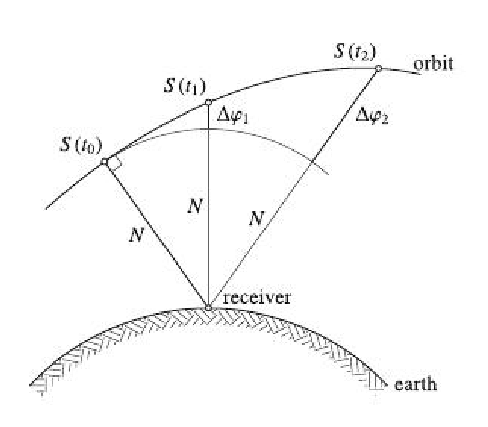
\includegraphics[scale=1.0]{ch2_measured_beat_phase.eps}
\caption{\textit{Geometryczna interpretacja obserwacji fazowych} źródło: \cite[][strona 108]{hofmann_gnss}}
\label{fig:receiver_beat_phase}
\end{figure}
Jeżeli podstawimy wyrażenie \ref{eq:receiver_beat_phase} do równania \ref{eq:beat_phase} oraz skorzystamy z zależności $f\lambda = c$,
otrzymamy następujące równanie \ref{eq:phase_pseldorange} fazowej psełdoodległości:
\begin{equation}
	\Phi = - \Delta{\varphi}_r^s\big|_{t_0}^{t} = \frac{\rho_r^s}{\lambda} + \frac{c}{\lambda} \big({\delta}t_r - {\delta}t^s\big) + N_r^s
	\label{eq:phase_pseldorange}
\end{equation}
Po pomnożeniu obu stron powyższego równania \ref{eq:phase_pseldorange} przez długość fali $\lambda$ oraz wprowadzjąc dodatkowe parametry opisujące wpływ błędów 
systematycznych oraz przypadkowych, otrzymujemy równanie \ref{eq:final_phase_equation} opisujące obserwacje fazowe w dziedzinie odległości ($[m]$).
Ze względu na charakter niniejszej pracy w równaniu uwzględniono tylko najważniejsze z opisanych w dalszej części błędów systematycznych.
\begin{equation}
	\lambda\Phi = \rho_r^s + c\big({\delta}t_r - {\delta}t^s\big) + {\lambda}N_r^s + {\delta}T_r^s 
	- {\delta}I_r^s + \epsilon
	\label{final_phase_equation}
\end{equation}
Występujące w powyższym równaniu nieoznaczoności $N_r^s$ są arbitralnymi liczbami całkowitymi unikalnymi dla każdego śledzonego przez odbiornik satelity.
Istnieją specjalne algorytmy pozwalające na estymowanie nieoznaczoności w dziedzinie liczb całkowitych, a tym samym na wyznaczanie pozycji anteny odbiornika
z bardzo wysoką dokładnościąrzędu centymetrów a w przypadku pomiarów statycznych nawet milimetrów.
Najczęściej jednak czas potrzebny na tzw. uzyskanie zbierzności rozwiązania jest 
dłuższy niż 15 minut w pomiarach absolutnych (PPP). W przypadku pomiarów różnicowych (RTK) korzystających z dwóch częstotliwości sygnału GNSS czas potrzebny 
na estymację nieoznaczoności w dziedzinie liczb całkowitych to średnio kilkadziesiąt sekund.\newline
\indent Błędy występujące w obserwacjach GNSS zarówno kodowych jak i fazowych dzielą się na przypadkowe, których nie można wyeliminować oraz na 
systematyczne, których wpływ można wyeliminować zupełnie lub w dużej mierze zredukować \cite[][strona]{hofmann_gnss}.
Źródła tych ostatnich dzielą się na trzy główne grupy \cite[][strona 109]{hofmann_gnss}:
\begin{itemize}
	\item Błędy związane z satelitami, takie jak błąd zegara oraz niedokładność orbity satelity.
	\item Błedy propagacji sygnału w atmosferze. Głównie refrakcja jonosferyczna oraz troposferyczna.
	\item Błedy odbiornika, do których należy błąd zegara, błąd położenia centrum fazowego anteny oraz błąd wielodrożności. 
\end{itemize}

	\subsection{DGPS/DGNSS}
	\subsection{RTK}
	\subsection{PPP}
\section{Nawigacja Inercjalna}
% w tej sekcji troche o filtrze kalmana 
%TODO trzeba opisać na czym polega filtracja Kalmana ( zaawansowane metody opracowania obserwacji)


\chapter{Algorytmy sterowania}
W pracy założono, że pojazdy rolnicze w przybliżeniu są bryłami sztywnymi.
Obiekty te charakteryzują się w przestrzeni trójwymiarowej sześcioma stopniami swobody.
Jednym ze sposobów matematycznego opisu położenia tychże pojazdów w przestrzeni trójwymiarowej,
jest podanie współrzędnych środka ciężkości (x,y,z) oraz trzech parametrów kątowych: azymutu, odchylenia od poziomu w płaszczyźnie poprzecznej oraz podłużnej.\\
\indent Rysunek \ref{fig:general_scheme} przedstawia typowy schemat systemu automatycznego prowadzenia pojazdów. Sprzęt komputerowy najczęściej składa się z 
odbiornika GNSS bądź innego narzędzia do wyznaczania absolutnej pozycji, sensora mierzącego aktualny kąt skrętu kół pojazdu oraz hydrauliki uaktualniającej kierunek kół.
Na oprogramowanie składają się: moduł planowania tras, moduł obliczający pożądane zmienne sterujące na podstawie porównania aktualnej pozycji z pozycją teoretyczną,
moduł sterujący, który oblicza sygnał sterujący na podstawie porównania zmierzonych oraz pożądanych zmiennych sterujących i wysyła go do hydrauliki uaktualniającej
\cite[][strona 1097]{automation_in_agriculture}.

\begin{figure}[H]
\centering
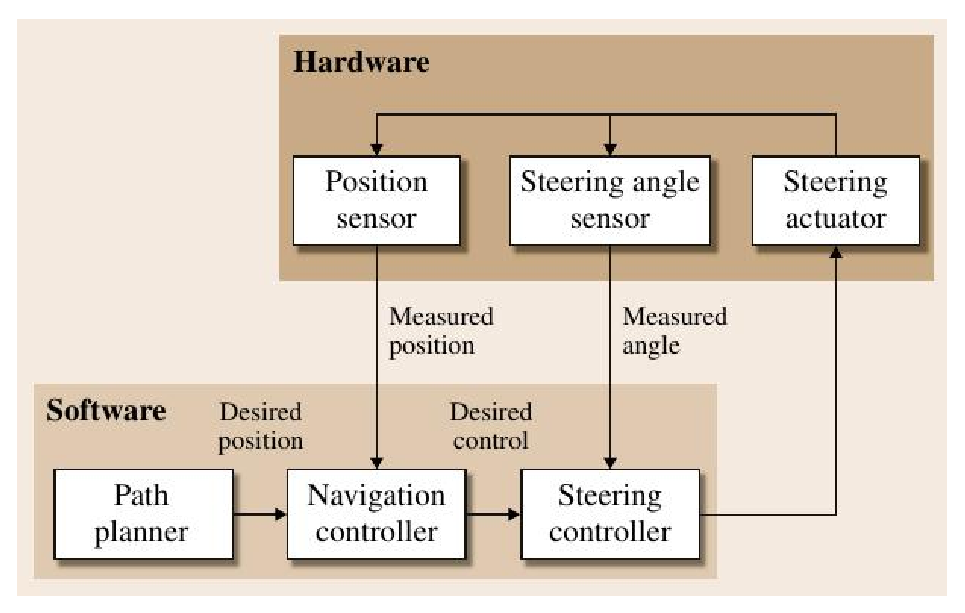
\includegraphics[scale=0.9]{ch3_general_scheme.eps}
\caption{\textit{Komponenty typowego systemu automatycznego prowadzenia}\\
źródło: \cite[][strona 1097]{automation_in_agriculture}}
\label{fig:general_scheme}
\end{figure}

\indent W dalszej części rozdziału opisano kilka przykładowych rozwiązań algorytmów sterowania,które charakterytzują się różnym podejściem 
w odniesieniu do parametrów kątowych określania orientacji przestrzennej pojazdów rolniczych. 
\section{Podział algorytmów sterowania ze względu na dostarczane dane wejściowe}
Jednym z najbardziej popularnych zbiorów parametrów nawigacyjnych oliczanych jako pożądane zmienne sterujące, które są następnie wysyłane do modułów sterowania, jest para:
azymut plus offset obliczane względem zadanej trasy. Azymut jest to kąt którego ramionami są:
główna oś symetrii pojazdu oraz styczna do krzywej prowadzenia w punkcie, który stanowi rzut prostopadły środka ciężkości na tą krzywą.
Offset natomiast jest to odległość środka ciężkości pojazdu względem zadanej ścieżki \cite{CCTA_769_775}.
Na rysunku nr \ref{fig:ch3_azymutOffset} przedstawione są powyższe parametry. Środek ciężkości pojazdu oznaczono jako C,
azymut pojazdu względem zadanej źcieżki oznaczono jako $\psi$. $\delta$ oznacza kąt sterujący jako wynik przetwarzania algorytmu sterującego tzw. Target Angle.    
\begin{figure}[H] 
\centering
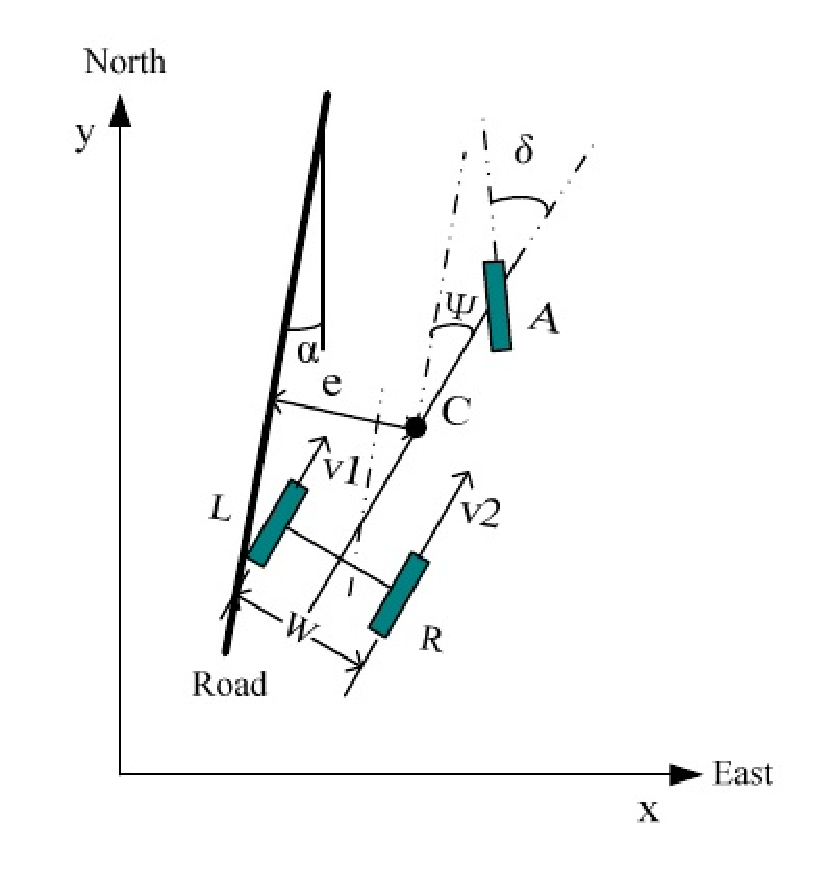
\includegraphics[scale=1.0]{ch3_azymutOffset.eps}
\caption{\textit{Azymut oraz offset - Parametry najczęściej używane w celu wyznaczenia pozycji względem zadanej trasy;}
źródło: \cite[][strona 464]{CCTA5_461_469}}
\label{fig:ch3_azymutOffset}
\end{figure}

W przypadku niskiej dokładności parametrów nawigacyjnych autorzy publikacji \cite{CCTA_943_950}
zaproponowali algorytm, który korzysta tylko z obliczanego w czasie rzeczywistym offsetu.
\begin{figure}[H]
\centering
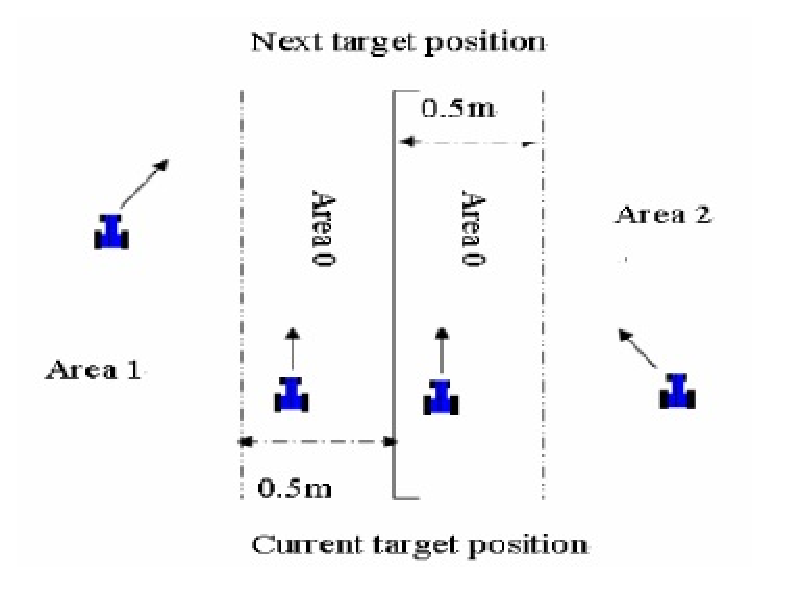
\includegraphics[scale=1.0]{ch3_currentNextTargetPosition.eps}
\caption{\textit{Tylko offset - w przypadku niskiej jakości danych wejściowych;}\\
	źródło: \cite[][strona 947]{CCTA_943_950}}
\label{fig:ch3_currentNextTargetPosition}
\end{figure}

\indent W przypadku trudnych warunków pogodowych bądź obecności innych czynników powodujących poślizg kół pojazdu wymagana 
jest estymacja współczynników korygujących wyniki algorytmu sterującego \cite[]{KRAUS}. Poniższy rysunek \ref{fig:side_forward_slip} ilustruje modelowanie 
poślizgu w płaszczyznach: poprzecznej oraz podłużnej.

\begin{figure}[H]
\centering
\begin{subfigure}{.4\textwidth}
  \centering
  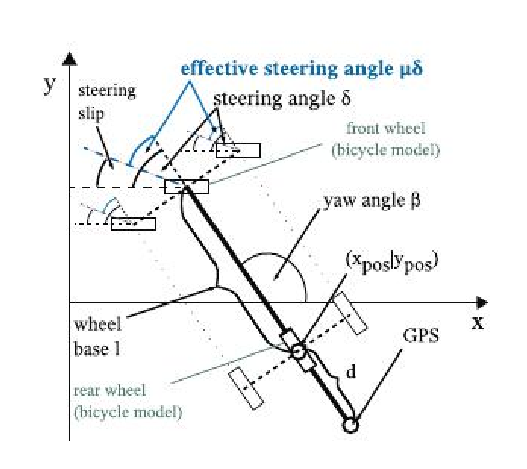
\includegraphics[width= 1.2\linewidth]{ch3_effective_stearing_angle.eps}
  \caption{Schemat przedstawiający zaadaptowanie modelu pojazdu jednosiowego z poślizgiem bocznym (w postaci zmiany kąta sterującego), do opisu ciągnika rolniczego}
  \label{fig:side_slip}
\end{subfigure}
\hspace{2cm}
\begin{subfigure}{.4\textwidth}
  \centering
  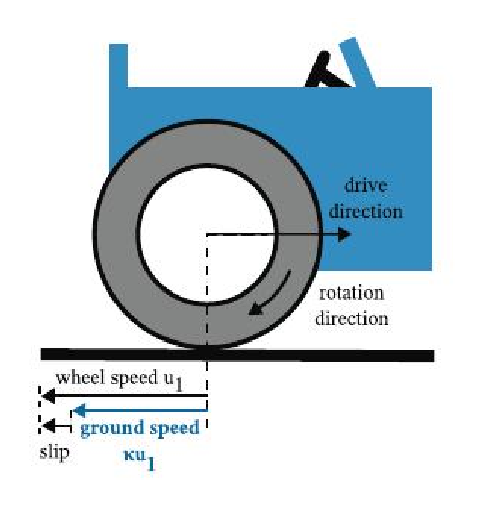
\includegraphics[width= 1.2\linewidth]{ch3_effective_wheel_speed.eps}
  \caption{Modelowanie poślizgu ciągnika w płaszczyźnie podłużnej}
  \label{fig:longitudinal_slip}
\end{subfigure}
\caption{\textit{Estymacja parametrów $\kappa$ oraz $\mu$ pozwalających na poprawne prowadzenie pojazdu w warunkach obecności poślizgu.}
źródło powyższych rysunków: \cite[][strona 26]{KRAUS}}
\label{fig:side_forward_slip}
\end{figure}

\section{Podział algorytmów sterowania ze względu na zastosowane algorytmy decyzyjne}
Różnego rodzaju algorytmy sterowania są używane w celu kompencacji zmiennej dynamiki pojazdów oraz w celu osiągnięcia satysfakcjonującej wydajności sterowania
 \cite[][strona 770]{CCTA_769_775}. Kilka kontrolerów zostało zaadaptowanych na potrzeby prowadzenia maszyn w rolnictwie precyzyjnym. Między innymi: 
Regulator proporcjonalno - całkująco różniczkujący PID\footnote{Proportional - Integral - Derivative controller}, wersja regulatora PID ze sprzężeniem zwrotnym\footnote
{feedback PID controller} oraz z predykcją\footnote{feedforward PID controller}, algorytmy logiki rozmytej oraz wiele innych \cite[][strona 1099]{automation_in_agriculture}.
Poniżej podano kilka przykładów wykorzystania różnych algortymów sterowania w rolnictwie.\\
\indent W pracy \cite[]{KRAUS} Tom Kraus wraz z współpracownikami opisali zaawansowany matematycznie algorytm wyznaczania parametrów prowadzenia 
ciągnika rolniczego - zmiany kąta sterowania oraz prędkości kątowej kół pojazdu, przy użyciu estymacji z przesówanym oknem czasowym (MHE\footnote{
Moving Horizon Estimation}) oraz nieliniowym modelem predykcyjnego sterowania (NMPC\footnote{Nonlinear Model Predictive Control}).
Wektor stanu poruszającego się obiektu, zawierający niewiadome $\kappa$, $\mu$ opisujące poślizg \ref{fig:side_forward_slip}, oraz orientację,
estymowany był za pomocą algorytmu MHE. Na podstawie znajomości aktualnego stanu obiektu oraz trasy referencyjnej algorytm predykcyjny NMPC wyznaczał wynikowe parametry 
prowadzenia pojazdu \cite[][strona 30]{KRAUS}. Rysunek \ref{fig:MHE_NMPC_diagram} przedstawia schemat blokowy opisanego algorytmu. 
Sterowanie predykcyjne z przesówanym oknem czasowym, polega na cyklicznym rozwiązywaniu zadania sterowania optymalnego, z warunkiem początkowym 
równym aktualnej estymacie stanu obiektu \cite[][strona 2]{BANIA}. Predykcja przyszłych stanów obiektu sterowanego na podstawie nieliniowych równań różniczkowych jest możliwa 
tylko w stosunkowo krótkim oknie czasowym przyjmowanym arbitralnie - stąd nazwa metody.
\begin{figure}[H]
	\centering
	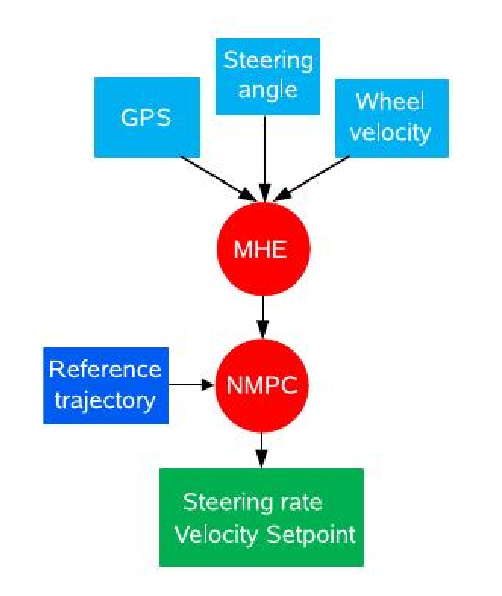
\includegraphics[scale = 0.9]{ch3_MHE_NMPC_estimation.eps}
	\caption{\textit{Schemat blokowy zaawansowanego algorytmu prowadzenia pojazdu dostosowanego do występowania poślizgu kół.}
	źródło \cite[][strona 30]{KRAUS}}
	\label{fig:MHE_NMPC_diagram}
\end{figure}

\indent W artykule \cite[]{feed_forward_back} Zhong-xiang Zhu oraz współpracownicy wykorzystali regulator proporcjonalno całkująco różniczkujący PID 
w obu wersjach zarówno ze sprzężeniem zwrotnym jak i z predykcją do znajdowania odpowiedniego kąta sterującego ciągnikiem rolniczym.
Podobnie jak w poprzedniej pracy powyżej, do opisu dynamiki pojazdu posłużono się modelem kinematycznym z uproszczonym podejściem jednoosiowym.
Kąt sterujący ${\alpha}_c$ obliczano jako sumę wartości predykowanej na podstawie teoretycznej trasy - wersja feedforward algorytmu PID, oraz korekty wynikającej 
z aktualnego połorzenia ciągnika - wersja ze sprzężeniem zwrotnym \cite[][strona 1599]{feed_forward_back}. 
\begin{equation}
	{\alpha}_c = {\alpha}_i^* + \delta\alpha
\end{equation}
Gdzie kąt ${\alpha}_{i}^{*}$ oznacza optymalny kąt sterujący wynikający z referencyjnego kursu, a $\delta\alpha$ jest poprawką obliczaną przez algorytm 
PID ze sprzężeniem zwrotnym na podstawie aktualnego azymutu pojazdu $\theta$ oraz offsetu $\delta\text{y}$, patrz rysunek \ref{fig:both_forward_back} poniżej.

\begin{figure}[H]
        \centering
        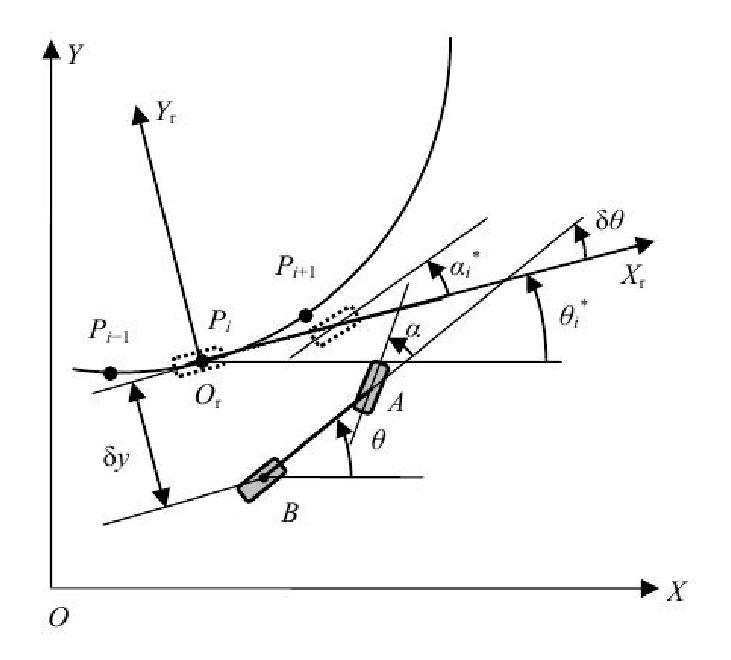
\includegraphics[scale = 1.0]{ch3_feedforward_plus_feedback.eps}
        \caption{\textit{Rysunek obrazujący model położenia pojazdu w świetle ścieżki referencyjnej}\\
        źródło \cite[][strona 1598]{feed_forward_back}}
        \label{fig:both_forward_back}
\end{figure}
Według autorów opracowania dokładność powyższego rozwiązania wyniosła średnio około $\pm$9cm na poziomie ufności 65\% \cite[][strona 1602]{feed_forward_back}.
Na koniec warto zauważyć, że w rozwiązaniu do wyznaczania azymutu pojazdu wykorzystano żyroskop światłowodowy o wysokiej dokładności (dryft $\pm$1.5\degree/h).
Zapewne dlatego otrzymano tak dobrą dokładność finalnego rozwiązania.



\chapter{Aktualne badania}
W przeciągu ostatniego ćwierćwiecza wynaleziono wiele technik oraz systemów służących do celów nawigacji: systemy satelitarne, systemy inercjalne,
systemy wizyjne oparte na przetwarzaniu obrazów cyfrowych w czasie rzeczywistym, radary wszelkiego typu.
Według panów Wan oraz Liu pojedynczy system dostarcza tylko częściowej informacji o środowisku zewnętrznym \cite[][strona 770]{CCTA_769_775}.
Ponadto dysponując tylko jednym narzędziem nie jest możliwa ocena jego wiarygodności. Z punktu widzenia statystyki matematycznej,
wiarygodność systemu, narzędzia, miernika jesteśmy w stanie określić wtedy i tylko wtedy gdy dysponujemy przynajmniej trzema niezależnymi od siebie źródłami danych.
Wtedy wykluczamy z opracowania błędne dane wejściowe. Ponadto im więcej posiadamy obserwacji danej wielkosći fizycznej tym większą jestesmy w stanie uzyskać dokładność.
Zatem pośrednio wyższa jest dokładność wyznaczenia pozycji oraz innych parametrów nawigacyjnych (kątowych)
w rozwiązaniach opartych na więcej niż jednym niezależnym źródle danych. W związku z powyższym systemy nawigacyjne oparte na fuzji obserwacji
pochodzących z kilku sensorów oraz systemów satelitarnych coraz bardziej zyskują na popularności \cite[][strona 770]{CCTA_769_775}
i prawdopodobnie w niedalekiej przyszłości zaczną dominować na rynku.
Pojedyncze obserwacje pochodzące z systemów GNSS charakteryzują się niską zmiennością ich dokładności w czasie.
Błąd wyznaczenia pozycji w przypadku rozwiązań kodowych pozostaje na niemalże stałym poziomie. 
W przypadku rozwiązań fazowych sytuacja jest podobna przy załorzeniu, że nie mamy utraty tzw. cykli fazowych.
Jeżeli jednak odbiornik utraci chociaż na moment sygnał do satelity, dokładność rozwiązania pogarsza się.
Nie spada jednak nigdy poniżej dokładności rozwiązania kodowego. Z poniższego rysunku wynika,
że obserwacje GNSS charakteryzują się mniejszą rozdzielczością czasową niż obserwacje INS,
ponadto mogą występować miejscowe pogorszenia dokładności lub w ekstremalnych przypadkach brak rozwiązania.
- trzeba porównać charakterystyki szeregów czasowych z ciekawych danych INS vs GNSS
GNSS – raczej nie wystepuja bledy systematyczne – brak dryftu, czasami dziury w rozwiazaniach, gorsza rozdzielczośc pomiarow. 
INS – dryft który narasta w czasie, wysoka rozdzielczosc pomiarow, brak dziór w obserwacjach,
Wniosek – integracja tych dwoch systemow jest super:)
TODO trzeba tutaj rysunek wstawic :)
\section{Zintegrowane systemy pozycjonowania w czasie rzeczywistym}
---zastosowanie zintegrowanego systemu pozycjonowania w precyzyjnym nawożeniu.
W artykule \cite{CCTA5_188_192} panowie Guobing Pan oraz Xiao Feng opisują zastosowanie zintegrowanego systemu bazującego na  systemie GPS w precyzyjnym nawozeniu roślin.
Nawożenie ma czterdziesto procentowy wpływ na wielkość plonowania. Ponadto szalenie ważny jest stopień wykorzystania dawki nawozu przez rośliny.
Dawkowanie nawozów charakteryzuje się zmiennością czasową związaną z różnymi etapami wzrostu rośliny oraz zmiennością przestrzenną w obrębie danego pola \cite{CCTA5_188_192}.
Zbyt niski współczynnik wykorzystania nawozu przez rośliny uprawne prowadzi do wzrostu kosztów produkcji 
oraz negatywnie wpływa na środowisko poprzez zanieczyszenie wód gruntowych.
W związku z powyższym  zmienny rozkład przestrzenny nawożenia wydaje się kluczowy do osiagnięcia wymiernych korzyści ekonomicznych \cite{CCTA5_188_192}.
Wedug autorów artykułu maszyny rolnicze powinny poruszać się według uprzednio zaprojektowanej trasy w celu automatyzacji oraz zwiększenia wydajności nawożenia.
Do realizacji systemu precyzyjnego nawożenia panowie Pan oraz Xiao za priorytet obrali minimalizację kosztów.
System zatem bazuje na kodowych obserwacjach GPS, które są zintegrowane za pomocą filteracji Kalmana
z azymutem pochodzącym z elektronicznego kompasu oraz z danymi z precyzyjnych akcelerometrów oraz z żyroskopów.
Zaprojektowany system najpierw na podstawie psełdoodległości GPS oblicza współrzędne w układzie WGS-84,
następnie transformuje uzyskaną pozycję do współrzędnych płaskich w odwzorowaniu Gaussa-Krugera.
Następnie na pdstawie danych z żyroskopu oraz kompasu elektronicznego otrzymujemy najbardziej prawdopodobny azymut.
Powyższe dane poddawane są następnie poddane obrubce filtrem Kalmana w celu obliczenia ostatecznej pozycji oraz orientacji pojazdu w przestrzeni.
Aktualna pozycja pojazdu oraz orientacja przestrzenna jest następnie wykorzystywana w celu obliczenia punktowej dawki nawozu
oraz korekty potrzebnej systemowi sterowania do prowadzenia według zadanej ścieżki.

---Zbieranie danych o glebie i jej właściwościach na potrzeby systemu precyzyjnego dawkowania nawozów 
opartego na technologi GIS przy użyciu systemu pozycjonowania GPS (DGPS, RTK)
Systemy nawigacji satelitarnej pomagają w zwiększeniu rozdzielczości oraz dokładności danych przestrzennych
dla potrzeb systemu dawkowania nawozów. Obecnie szybka akwizycja danych terenowych opisujących właściwości glebowo rolnicze pól uprawnych
stanowi ważny aspekt badań nad rozwojem rolnictwa precyzyjnego. Zwiększenmie rozdzielczoąci prubkowania jest możliwe dzięki
dynamicznemu rozwojowi nawigacji w czasie rzeczywistym (RTK, DGPS) zwłaszcza poprzez lokalne systemy stacji referencyjnych ASG-EUPOS.
Dla przykładu im wyższa jest rozdzielczość prubkowania, tym dokładniejsza jest interpolacja danych 
(ph, fizyko chemiczne właściwości gleby itp, określana przez system GIS) na potrzeby określania dawek nawozów.
Posumowując ten artykuł: Dane przestrzwenne zbierane były za pomocą DGPS z wykorzystaniem lokalnych stacji referencyjnych.
Następnie wyniki pomiarów parametrów glebowych były wprowadzane do GIS-owej bazy danych. Na podstawie zebranych danych były tworzone mapy nawożenia \cite{CCTA5_268_278}.

---Tani System równoległego prowadzenia pojazdów rolniczych oparty na filtrze Kalmana.
Prowadzenie równoległe jest jedną z najbardziej popularnych obecnie metod ułatwiających prace polowe.
W pracy \cite{CCTA5_461_469} czytamy, że przeprowadzono już wiele badań nad zastosowaniem bardzo dokładnych odbiorników fazowych RTK-GPS
przy automatyzacji maszyn rolniczych. Autorzy twierdzą jednak, że koszt precyzyjnych odbiorników GPS jest zbyt wysoki
i nie pozwala na ich powszechną adaptację w rolnictwie. Ponieważ, zintegrowane systemy nawigacyjne oparte na filtrze Kalmana
znacznie podnoszą dokładność pozycjonowania, a technologia czujników elektronicznych bardzo szybko się rozwija,
możliwa jest zatem konstrukcja tanich systemów pozycjonowania atrakcyjnych pod względem zastosowania ich w rolnictwie precyzyjnym \cite{CCTA5_461_469}.
Panowie Zhang, Feng, Li, Rao oraz Di Cui skonstruowali zintegrowany system do równoległego prowadzenia złożony z odbiornika DGPS,
z elektronicznych żyroskopów MEMS, z dwóch czujników prędkości oraz z precyzyjnego potencjometru do pomiaru skrętu kół.
Schemat blokowy omawianego systemu przedstawiono na rysunku \ref{fig:ch4_multisensorSystem}.
Dane z poszczególnych podzespołów przesyłane były do komputera z systemem wbudowanym na którym zainstalowano Filtr Kalmana.
Całkowity koszt systemu wyniósł w przybliżeniu około 1500\$.
\begin{figure}[H]
\centering
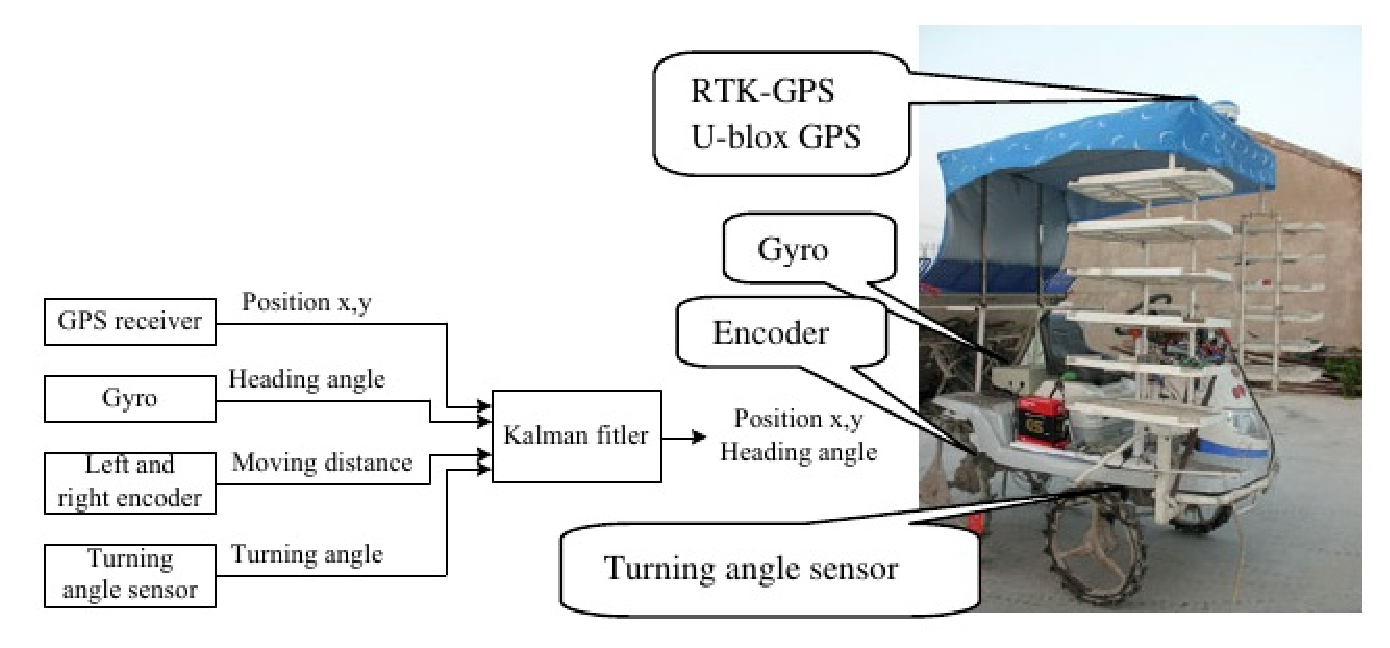
\includegraphics[width=\textwidth]{ch4_multisensorSystem.eps}
\caption{\textit{Przykład zintergrowanego systemu do równoległego prowadzenia;} 
źródło: \cite[][strona 464]{CCTA5_461_469}}
\label{fig:ch4_multisensorSystem}
\end{figure}   
RTK-GPS był używany jako odniesienie w celu porównania otrzymanych wyników. 
Współrzędne w lokalnym układzie odniesienia, azymut, oraz prędkość były zadane jako wektor stanu w filtrze Kalmana.
Wyniki eksperymentu pokazały, że obróbka danych przestrzennych za pomocą filtru Kalmana znacznie podnosi dokładność wspólrzędnych DGPS.
Średnie residua w odniesieniu do pozycji RTK zostały zredukowane z 2.21m do 0.52m względem osi x oraz z 0.68m do 0.23m względem osi y.
Jednakże zaimplementowany algorytm nie usunął całkowicie błędów systematycznych zawartych w danych DGPS.
Maksymalna odchyłka od równoegłości po przebyciu 70 m wyniosła 3m \cite{CCTA5_461_469}.

--- Integracja danych RTK-GPS z elektronicznym kompasem oraz obrazowaniem cyfrowym z urzyciem logiki rozmytej (Fuzzy logic).
W artykule pod tytułem “Automatic Navigation System With Multiple Sensors” panowie Wan oraz Liu
opisali system automatycznego prowadzenia pojazdów rolniczych bazujący na integracji obserwacji pochodzących z elektronicznego kompasu,
odbiornika GPS oraz kamery cyfrowej z matrycą CCD. W celu obliczenia parametrów prowadzenia pojazdu względem zadanej trasy,
dane z wszystkich powyższych mierników były przetwarzane z użyciem narzędzi logiki rozmytej tzw. Fuzzy Logic.
Poniżej na rysunku nr \ref{fig:ch4_fuzzyLogic} przedstawiono diagram blokowy opisujący algorytm integracji danych.
\begin{figure}[H]
\centering
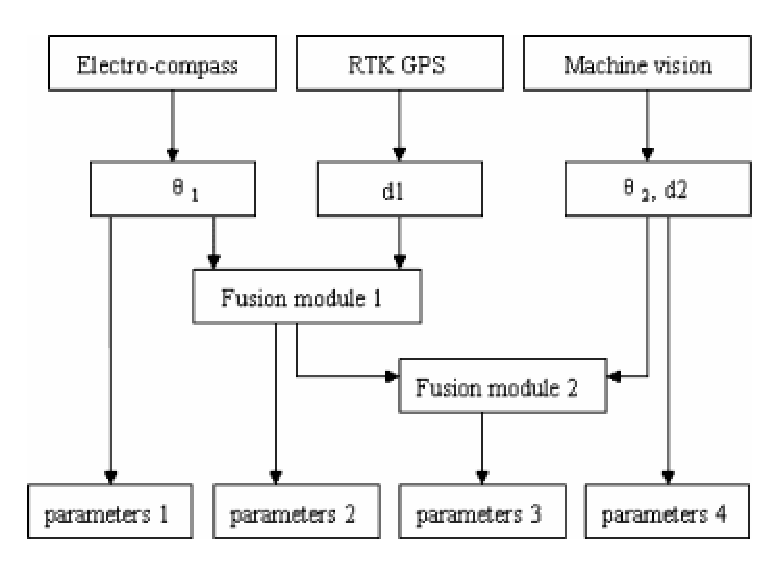
\includegraphics[width=8cm, height=7cm]{ch4_fuzzyLogic.eps}
\caption{\textit{Zastosowanie narzędzi logiki rozmytej do integracji danych nawigacyjnych;}
źródło: \cite[][strona 774]{CCTA_769_775}}
\label{fig:ch4_fuzzyLogic}
\end{figure}

Azymut kierunku jazdy względem zadanej ścieżki oraz ofset oznaczono odpowiednio jako $\theta$ oraz d.
Wszystkie powyższe rezultaty pośrednie zanim przesłano do modułów logiki rozmytej przetransformowano do układu obrazu cyfrowego,
w celu zapewnienia jednolitego układu odniesienia. Jako ostateczną i najbardziej prawdopodobną wersję parametrów $(d, \theta )$
przyjęto wyniki z modułu numer 2 (parameters 3), pozostałe rezultaty posłużyły do wybrania jak najlepszych współczynników skalowania obserwacji
w modułach wykorzystujących logikę rozmytą. Na podstawie parametrów określających położenie pojazdu względem zdefiniowanej uprzednio trasy
obliczany był teoretyczny kąt skrętu kół, przekazywany następnie do realizacji w układzie sterującym (target angle), patrz rysunek \ref{fig:ch4_fuzzyLogicTargetAngle}.
\begin{figure}[H]
\centering
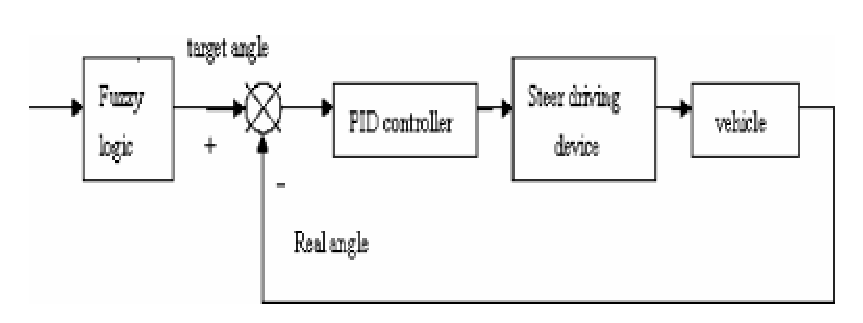
\includegraphics[height=4cm]{ch4_fuzzyLogicTargetAngle.eps}
\caption{\textit{Schemat algorytmu znajdującego odpowiedni kąt skrętu kół pojazdu rolniczego;}
	źródło: \cite[][strona 775]{CCTA_769_775}}
\label{fig:ch4_fuzzyLogicTargetAngle}
\end{figure}
System sterujący realizował swoje zadania w oparciu o algorytm PID - regulator proporcjonalno-całkująco - różniczkujący.
Według autorów pracy \cite{CCTA_769_775} opisany system spełnia wymagania automatycznego prowadzenia maszyn rolniczych w warunkach roboczych.
\section{Spegcjalistyczne opracowanie obserwacji - postprocessing}
--- szczególnie ważny z punktu widzenia opracowania map plonowania.
Pan Xiaochao Zhang wraz z zespołem w artykule \cite{CCTA_951_958} opisali konstrukcję systemu służącego do tworzenia map plonowania.
Głównym elementem systemu był poziomo umieszczony czujnik mierzący masę przepływającego ziarna.
Surowe wyniki były poprawiane ze względu na wilgotność, a następnie zamieniane na ilość ziarna przez algorytm całkujący.
Mapa plonu była tworzona przy wykorzystaniu danych przestrzennych z odbiornika GPS, po uprzedniej synchronizacji czasowej.
W celu zwiększenia dokładności mapowania obserwacje GPS były poddane specjalistycznemu opracowaniu tzw. Postprocessing,
zanim zintegrowano je z danymi plonowania. Ostateczne wyniki podczas testów charakteryzowały się błędem względnym na poziomie 3.5\%. 
Poniższy rysunek \ref{fig:ch4_creatingPlantsMap} przedstawia działający system w trybie operacyjnym.
\begin{figure}[H]
\centering
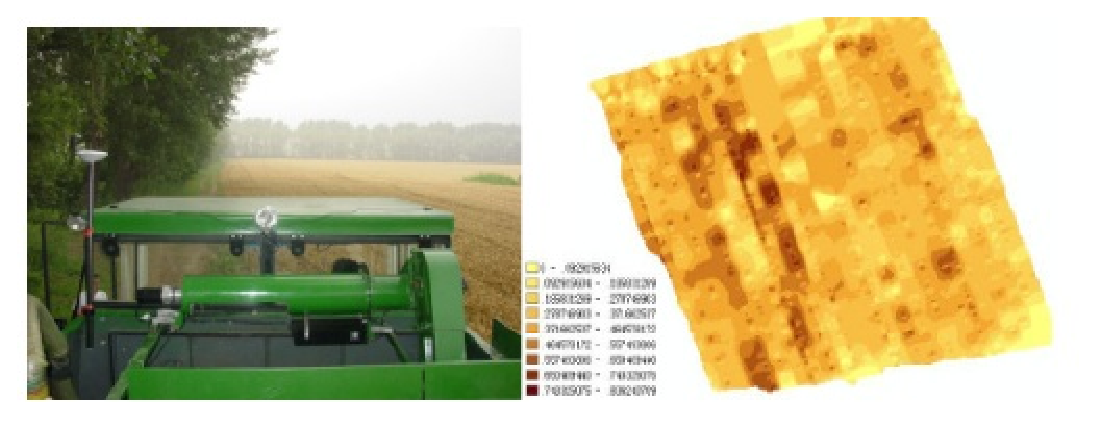
\includegraphics[width=\textwidth]{ch4_creatingPlantsMap}
\caption{\textit{System do tworzenia map plonowania;} źródło: \cite[][strona 954]{CCTA_951_958}}
\label{fig:ch4_creatingPlantsMap}
\end{figure}
Mapy plonów są ważnym źródłem informacji dla rolników. Pomagają w planowaniu zabiegów agrotechnicznych.

\section{Inne zastosowania GNSS w rolnictwie precyzyjnym}
--- pomiary pól powierzchni na potrzeby rolnictwa precyzyjnego
	( Computer and Computing Technologies in Agriculture; volume 2; s. 993)

--- zastosowanie GPS w automatycznym zmiennym nawadnianiu 
Celem precyzyjnego nawadniania jest minimalizacja użycia zasobów wodnych, przy załorzeniu  spełnienia w jak największym stopniu wymagań roślin uprawnych.
Dystrybucja przestrzenna wymagań roślinnych względem ilości dodatkowego nawadniania, zależy głównie od warunków glebowych oraz topografii terenu.
Dlatego zasadnym jest przeprowadzanie nawadniania pól uprawnych, zgodnie z wcześniej sporządzanymi mapami docelowego rozkładu przestrzennego dawek H2O 
\cite{PA_RemoteIrrigation}.
\begin{figure}[H]
\centering
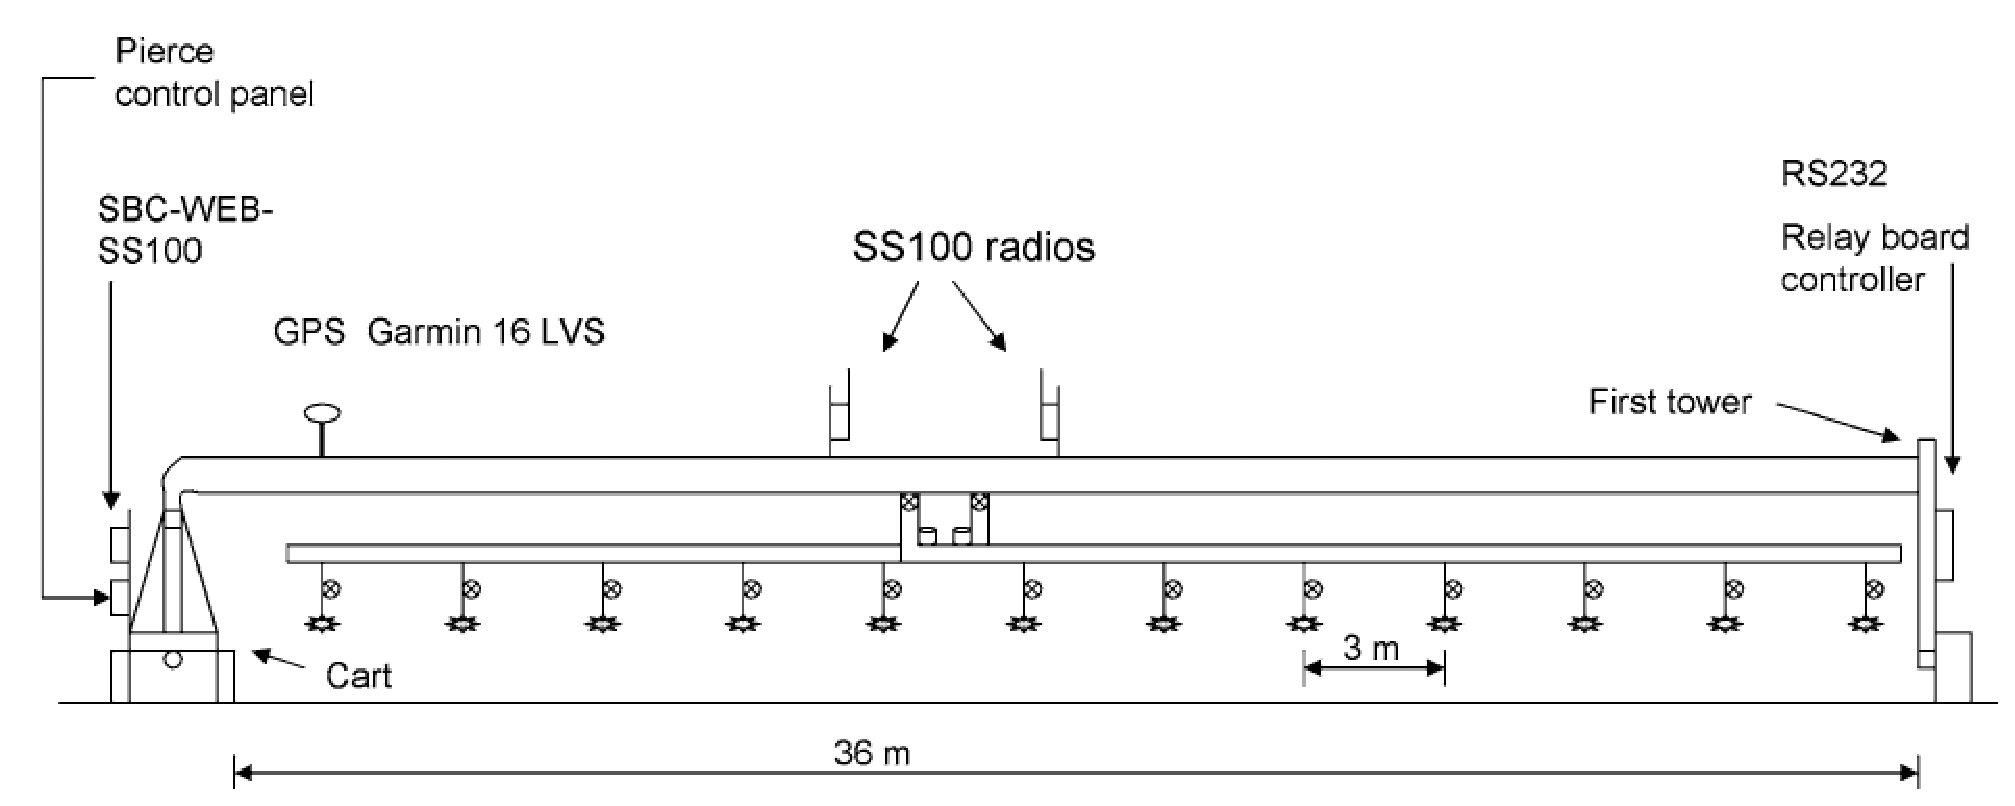
\includegraphics[width=\textwidth]{ch4_remoteIrigationMonitoring}
\caption{\textit{Schemat systemu służącego do automatycznego nawadniania pól uprawnych;} źródło: \cite[][strona 04]{PA_RemoteIrrigation}}
\label{fig:ch4_remoteIrigationMonitoring}
\end{figure}
Jose L. Chavez i wsp. w artykule \cite{PA_RemoteIrrigation} zaprojektowali system precyzyjnego nawadniania, sterujący niezależnie poszczególnymi dyszami,
których przepływ determinowano w oparciu o mapy nawadniania. Na rysunku \ref{fig:ch4_remoteIrigationMonitoring} przedstawiono schemat systemu.
Z punktu widzenia niniejszego opracowania najważniejszym elementem systemu jest odbiornik GPS umieszczony precyzyjnie nad pierwszą dyszą,
który pozwala na określenie jej pozycji przestrzennej i obliczenie dawki H2O. Położenie kolejnych dysz określano za pomocą translacji
o zadany wektor względem pierwszej, przy załorzeniu, że ramię systemu jest zawsze prostopadłe do kierunku ruchu.
Mapy nawadniania tworzone były na podstawie danych o wilgotności gleby oraz powietrza zbieranych za pomocą sieci czujników
równomiernie rozmieszczonych na polu uprawnym. 







\chapter{Analiza rynku}
W tym rozdziale przedstawiono przykłady systemów, narzędzi oraz technik nawigacyjnych, które są wykorzystywane w usługach firm komercyjnych 
oraz w dostarczanych przez te firmy systemach rolnictwa precyzyjnego. Z uwagi na niską dostępność specyfikacji technicznych produktów 
dostępnych obecnie na rynku, w pracy ogranioczono się do analizy ofert marketingowych liderów branży maszyn rolniczych.
Jako reprezentatywną próbę dla europejskiego rynku rolnictwa precyzyjnego przyjęto oferty następujących firm: New Holland Agriculture,
John Deere oraz Claas.
\section{Wykorzystanie GNSS}
% test cytowania \cite{CLAAS_stearing_systems}\\
%	test cytowania \cite{JOHN_DEERE_solutions}\\
%	test cytowania \cite{NEW_HOLLAND_PLM}
W tym podrozdziale w formie porównania wykorzystywanych systemów pozycjonowania a także oferowanych technik wyznaczania pozycji opisano wykorzystanie 
systemów GNSS przez firmy komercyjne z grupy wybranej jako reprezentatywna.\\
\indent Na wstępie należy uściślić pojęcia dokładności, które pojawiały się w broszurach marketingowych, a które nie zawsze były rzetelnie opisywane 
przez firmy refereujące o swoich produktach. Z reguły gdy w broszurach podawana jest dokładność, brakuje informacji odnośnie poziomu ufności\footnote{
W przypadku wyznaczania pozycji poziom ufności bezpośrednio określa prawdopodobieństwo zawarcia wartości prawdziwej (prawdziwe położenie) w okręgu o środku w punkcie 
estymowanym i promieniu równym odpowiednio: 1$\sigma$ P=68\%; 2$\sigma$ P=95\%; 3$\sigma$ P=99.7\%, gdzie $\sigma$ oznacza odchylenie standardowe estymowanej pozycji.}
oraz czy jest to dokładność w sensie absolutnym czy może dokładność podawana jest relatywnie w stosunku do kolejnych wyznaczeń tym samym odbiornikiem - tzw.
dokładnośc między-przejazdowa (pass to pass accuracy). Typ uzyskiwanej dokładności - relatywna czy absolutna rzutuje bezpośrednio na rodzaj zabiegów 
agrotechnicznych, które możemy wykonywać. Dla przykładu przy zakładaniu ścieżek przejazdowych, które mają służyć przez cały sezon wegetacyjny potrzebna 
jest wysoka dokładność w sensie absolutnym, natomiast w celu eliminacji omijaków bądź nakładek przy zabiegach agrotechnicznych wystarczy dokładność między-przejazdowa.
Aby uniknąć nieporozumień nacisk połorzono na porównanie wykorzystywanych technologii. Wszędzie tam gdzie w broszurach marketingowych nie wyspecyfikowano typu 
dokładności w pracy zamieszczono oba rodzaje zaczerpnięte z literatury lub strony producenta.\\
\indent Wszystkie trzy firmy oferują w swoim portfolio odbiorniki mające możliwość odbioru sygnału zarówno GPS jak i GLONASS w dwóch częstotliwościach.
Firma John Deere ma w swojej ofercie odbiornik StarFire 3000 rysunek \ref{fig:john_deere_starfire}. Firma Class oferuje Antenę GPS PILOT wraz z terminalem S7
\ref{fig:class_antena} i komputerem nawigacyjnym przedstawionym na rysunku \ref{fig:class_navigation_computer}, natomiast 
firma New Holland Agriculture w swojej ofercie prezentuje kilka rodzajów anten oraz odbiorników w zależności od wymaganej dokładności. Przykładem jest odbiornik 
NH 372 przedstawiony na rysunku \ref{fig:new_holland_nh372}.
\begin{figure}[H]
\centering
        \begin{subfigure}{0.3\textwidth}
                \centering
                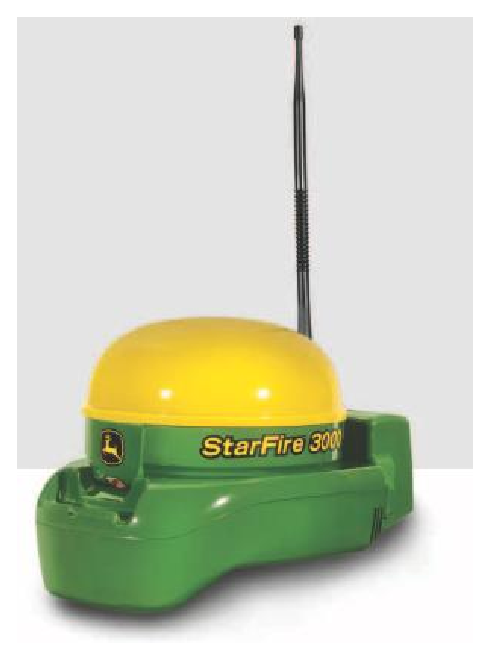
\includegraphics[width=0.9\linewidth]{ch5_john_deere_starfire.eps}
                \caption{Odbiornik StarFire 3000 firmy John Deere}
                \label{fig:john_deere_starfire}
        \end{subfigure}
        %\hfill
        \begin{subfigure}{0.3\textwidth}
                \centering
                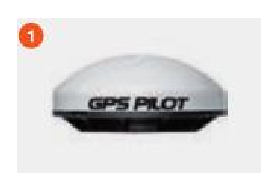
\includegraphics[width=0.9\linewidth]{ch5_class_antena.eps}
                \caption{antena GPS PILOT firmy Class}
                \label{fig:class_antena}
        \end{subfigure}
        \begin{subfigure}{0.3\textwidth}
                \centering
                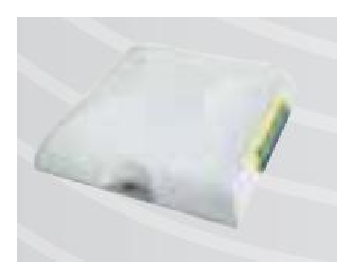
\includegraphics[width=0.9\linewidth]{ch5_new_holland_receiver.eps}
                \caption{odbiornik NH 372 firmy New Holland Agriculture}
                \label{fig:new_holland_nh372}
        \end{subfigure}
\caption{Przegląd komercyjnych odbiorników GNSS}
\end{figure}
%%%%%%%%%%%%%%%%%%%%%%%%%%%%EGNOS%%%%%%%%%%%%%%%%%%%%%%%%%%%%%%%%%%%%%%%%%%
\indent Jeżeli weźmiemy pod uwagę publicznie dostępne systemy augmentacyjne GNSS, to europejski system EGNOS jest wykorzystywany 
przez firmy Class oraz New Holland Agriculture. Ponadto firm New Holland oferuje zbliżony dokładnością do systemu EGNOS sygnał korekcyjny OmniStar VBS rysunek
\ref{fig:omnistar_vbs}. Firma John Deere dostarcza swojego własnego rozwiązania w postaci sygnału 
korekcyjnego SF1. Absolutna dokładność rozwiązania GNSS z sygnałem korekcyjnym EGNOS jest na poziomie trzech metrów (2$\sigma$).
Ponieważ, firmy zalecają używanie GNSS z sygnałem korekcyjnym EGNOS do prowadzenia prac uprawowych, w których powtarzalność przejazdów nie 
ma istotnego znaczenia, zatem w ofercie prezentują dokładność relatywną na poziomie $\pm$30cm. Relatywna dokładność GNSS z sygnałem korekcyjnym SF1 od John Deere 
jest podawana na poziomie $\pm$23cm. System EGNOS transmituje poprawki różnicowe dla częstotliwości L1 sygnału GPS za pomocą łącza satelitarnego. Działanie systemu 
przedstawia poniższy rysunek \ref{fig:class_egnos}.
\begin{figure}[H]
\centering
        \begin{subfigure}{0.4\textwidth}
                \centering
                
\includegraphics[width=0.9\linewidth]{ch5_new_holland_egnos.eps}
                \caption{\textit{Zasięg sygnału OmniStar VBS} źródło \cite[][strona 4]{NEW_HOLLAND_PLM}}
                \label{fig:omnistar_vbs}
        \end{subfigure}
        \begin{subfigure}{0.4\textwidth}
                \centering
                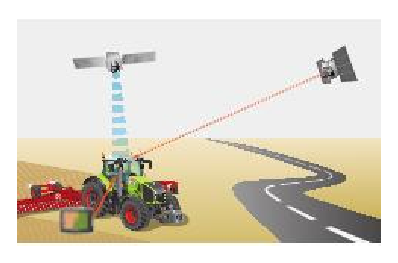
\includegraphics[width=0.9\linewidth]{ch5_class_egnos.eps}
                \caption{\textit{Zasada działania systemu EGNOS według Class} źródło \cite[][strona 26]{CLAAS_stearing_systems}}
                \label{fig:class_egnos}
        \end{subfigure}
\caption{Wykorzystanie sygnału korekcyjnego niskiej jakości}
\end{figure}
\indent 

\section{Zastosowanie systemów inercjalnych}
Na podstawie analizy ofert marketingowych firm z grupy przyjętej za referencyjną, można wywnioskować, że systemy nawigacji inercjalnej 
są wykorzystywane na potrzeby budowy systemów służących do kompensacji nierówności terenu przy precyzyjnym prowadzeniu maszyn rolniczych.
Firma Trimble w swoich technologiach kompensacji terenu T2, T3 wykorzystuje akcelerometry do wyznaczania kąta inklinacji\footnote{kąt zawarty między osią 
pionową pojazu a kierunkiem siły ciężkości w danym punkcie na Ziemi.} oraz żyroskopy w celu kompensacji danych z akcelerometrów ze względu na własną dynamikę pojazdu oraz 
w celu wyznaczania prędkości z jaką zmienia się położenie pojazdu względem kierunku pionu \cite[]{TRIMBLE}.
Z analizowanej grupy firma John Deere oferuje autorskie rozwiązania w postaci modułu kompensacji terenu TCM. Moduł TCM pozwala na wprowadzanie korekt 
do pozycji GNSS ze względu na pochyłości terenu w trzech osiach z, y, z. Moduł kompensacji terenu jest domyślenie zintergrowany z odbiornikiem GNSS StarFire 3000.
Rysunek \ref{fig:john_deere_tcm} przedstawia możliwości systemu TCM. 

\begin{figure}[H]
\centering
\begin{minipage}[c]{0.6\linewidth}
  \begin{flushleft}
  	\begin{minipage}[t]{0.5\linewidth}
		\raggedleft
		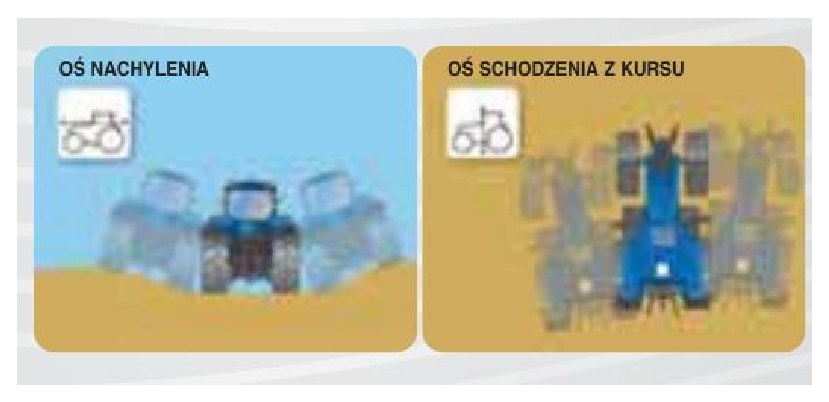
\includegraphics[scale = 0.4]{ch5_new_holland_terrain_compensation_t2.eps}	
		\subcaption{Technologia kompensacji terenu T2 wykorzystywana przez New Holland Agriculture}
		\label{fig:t2}
	\end{minipage}
	\vfill
	\begin{minipage}[b]{0.5\linewidth}
		\raggedleft
		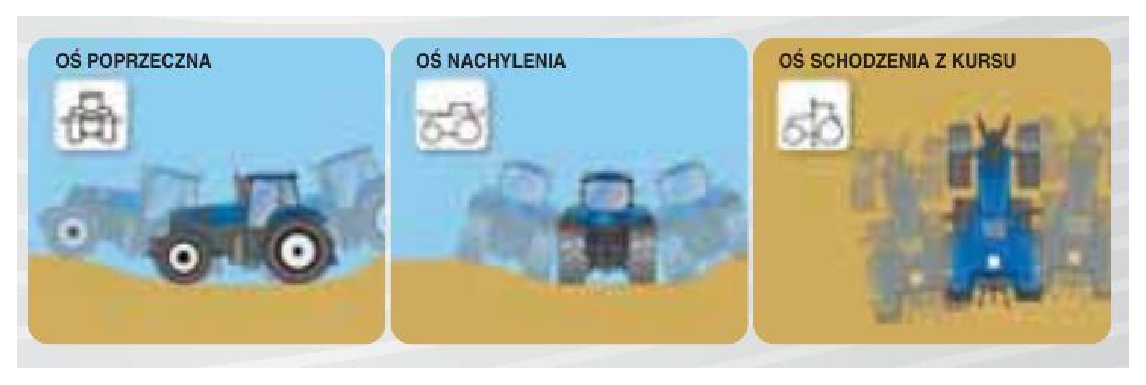
\includegraphics[scale = 0.4]{ch5_new_holland_terrain_compensation_t3.eps}
		\subcaption{Technolohia kompenasacji terenu T3 wykorzystywana przez New Holland Agriculture}
		\label{fig:t3}
	\end{minipage}
  \end{flushleft}
\end{minipage}%
\hfill
\begin{minipage}[c]{0.4\linewidth}
  \begin{flushright}
  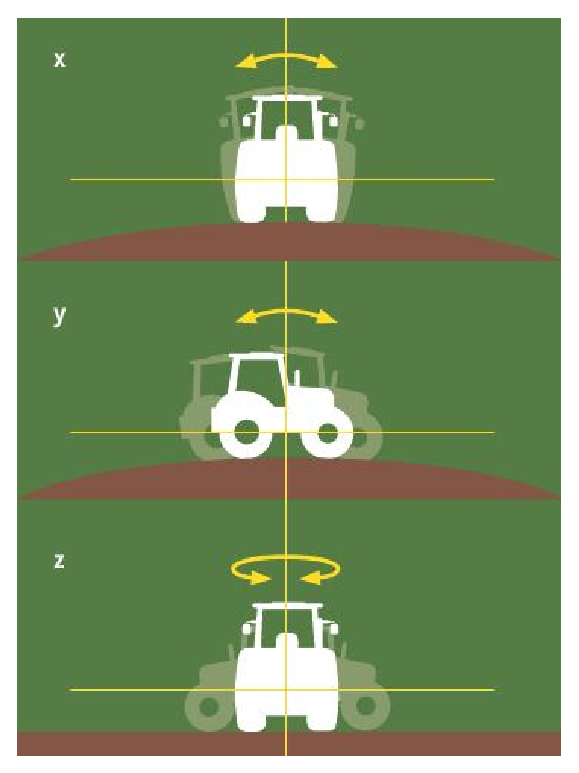
\includegraphics[scale = 0.5]{ch5_john_deere_terrain_compensation.eps}
  \subcaption{\textit{Technologia kompensacji terenu TCM od John Deere} źródło \cite[][strona 8]{JOHN_DEERE_solutions}}
  \label{fig:john_deere_tcm}
  \end{flushright}
\end{minipage}
\caption{\textit{Kompensacja wpływu nierówności terenu na pozycję GNSS}}
\label{fig:terrain_compensation}
\end{figure}
Firma New Holland Agriculture również posiada w swojej ofercie system kompensacji terenu w dwóch różnych wersjach: T2 - z pominięciem kompensacji w 
płaszczyźnie podłużnej, T3 - kompensujący nierówności w obu płasczyznach (poprzeczna, podłużna) oraz zapobiegający schodzeniu maszyny z kursu \cite[][strona 7]{NEW_HOLLAND_PLM}.
Firma New Holland Agriculture najprawdopodobniej wykorzystuje rozwiązania T2 oraz T3 oferowane przez odbiorniki marki Trimble. 
Na rysunku \ref{fig:t2} oraz \ref{fig:t3} przedstawiono schemat działania rozwiązań zaadoptowanych przez New Holland.
Firma Class w swoim portfolio również posiada 6 osiowy żyroskop (żyroskop akcelerometr) do uwzględniania ruchów podłużnych i poprzecznych pojazdu. 
Moduł INS jest wmontowany w specjalny komputer nawigacyjny - rysunek \ref{fig:class_navigation_computer}, 
który wylicza ślady przejazdów oraz wprowadza korekty ze względu na nierówności terenu.\\
\begin{figure}[H]
	\centering
	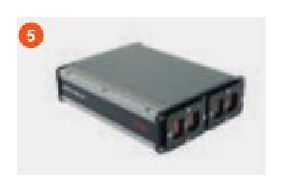
\includegraphics[scale=0.4]{ch5_class_navigation_computer.eps}
	\caption{Komputer do nawigacji Class z wmontowanymi sensorami do kompensacji nierówności terenu}
	\label{fig:class_navigation_computer}
\end{figure}
\indent Warto nadmienić, że firmy obecnie jedynie wykorzystują narzędzia nawigacji inercjalnej (INS) do korekcji rozwiązań GNSS.
Z broszur marketingowych wywnioskować można, że komercyjnie nie stosuje się jeszcze filtru kalmana w celu wspólnego opracowania obserwacji GNSS plus INS.
\section{Zastosowanie sensorów video}
Firma CLASS w swojej ofercie posiada systemy wspomagające nawigację GNSS oparte o sensory wideo. CAM PILOT przedstawiony na rysunku \ref{fig:class_cam_pilot1}
jest systemem automatycznego kierowania sterowanym przez kamerę stereoskopową. Został zaprojektowany specjalnie do zbioru traw. Kamera ustala pozycję pokosów 
i na podstawie tej informacji odbywa się prowadzenie pojazdu \cite[][strona 7]{CLAAS_stearing_systems}.
W ofercie firmy CLASS jest także system oparty na skaningu laserowym LASER PILOT zobrazowany na 
rysunku \ref{fig:class_laser_pilot1} zaprojektowany do ustalania krawędzi między polem skoszonym a jeszcze nie omłuconym. System pozwala na 
prowadzenie pojazdu wzdłuż tej krawędzi z dokładnością 10-20cm \cite[][strona 6]{CLAAS_stearing_systems}.
\begin{figure}[H]
\centering
	\begin{subfigure}{0.4\textwidth}
		\centering
		
\includegraphics[width=0.9\linewidth]{ch5_class_cam_pilot0.eps}
		\caption{CLASS CAM PILOT}
		\label{fig:class_cam_pilot1}
	\end{subfigure}
	%\hfill
	\begin{subfigure}{0.4\textwidth}
                \centering
                
\includegraphics[width=0.9\linewidth]{ch5_class_laser_pilot0.eps}
                \caption{CLASS LASER PILOT}
                \label{fig:class_laser_pilot1}
	\end{subfigure} \\
	\vfill
	\begin{subfigure}{0.4\textwidth}
                \centering
                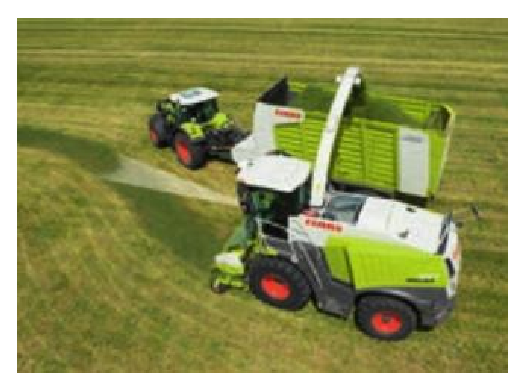
\includegraphics[width=0.9\linewidth]{ch5_class_cam_pilot.eps}
                \caption{CLASS CAM PILOT podczas pracy}
                \label{fig:class_cam_pilot2}
	\end{subfigure}
	\begin{subfigure}{0.4\textwidth}
                \centering
                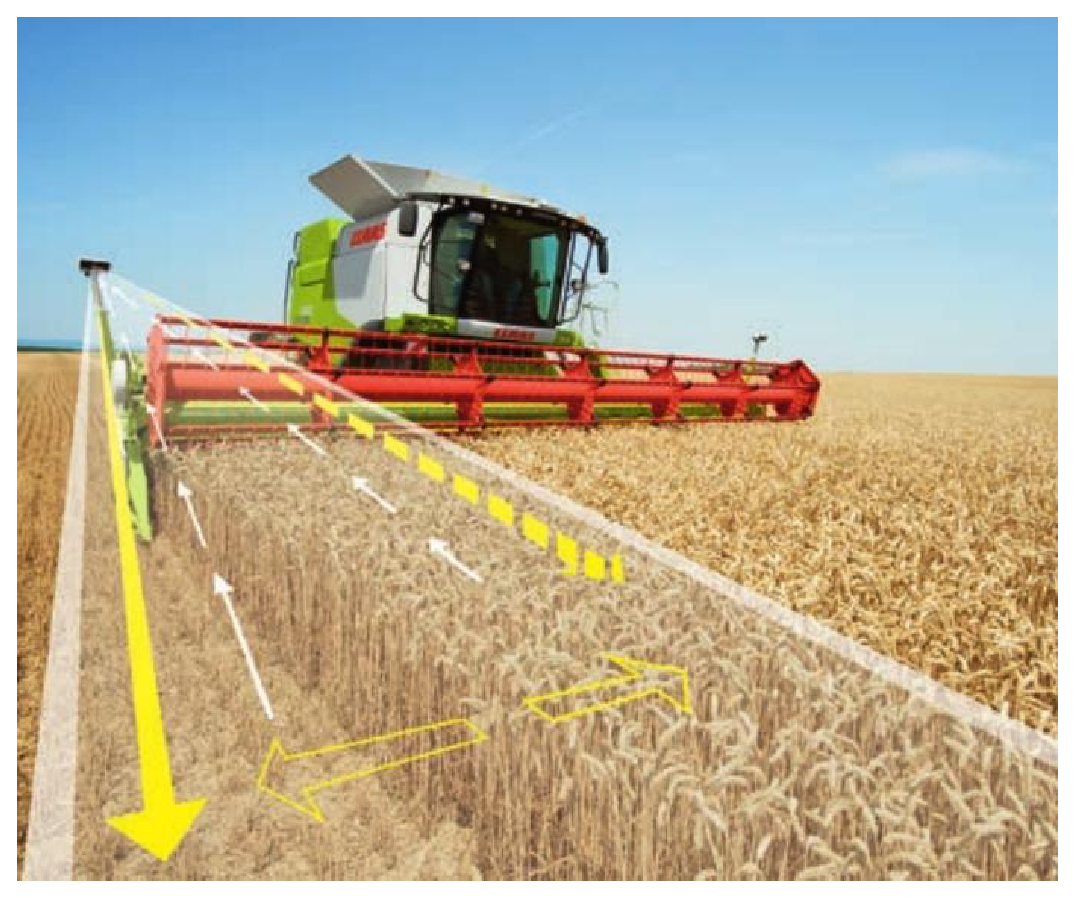
\includegraphics[width=0.9\linewidth]{ch5_class_laser_pilot.eps}
                \caption{CLASS LASER PILOT podczas pracy}
                \label{fig:class_laser_pilot2}
	\end{subfigure}
\caption{Systemy bazujące na sensorach wideo marki CLASS}
\end{figure}
\indent Również firma New Holland Agriculture posiada w swej ofercie system oparty na sensorach wideo.
System SMARTSTEER przedstawiony na rysunku \ref{fig:new_holland_smartsteer} za pomocą skanera laserowego wytycza krawędź dzielącą ściernisko 
od zborza i na podstawie tej informacji przesyła sygnały do układu kierowniczego \cite[][strona 18]{NEW_HOLLAND_PLM}.
\begin{figure}[H]
	\centering
	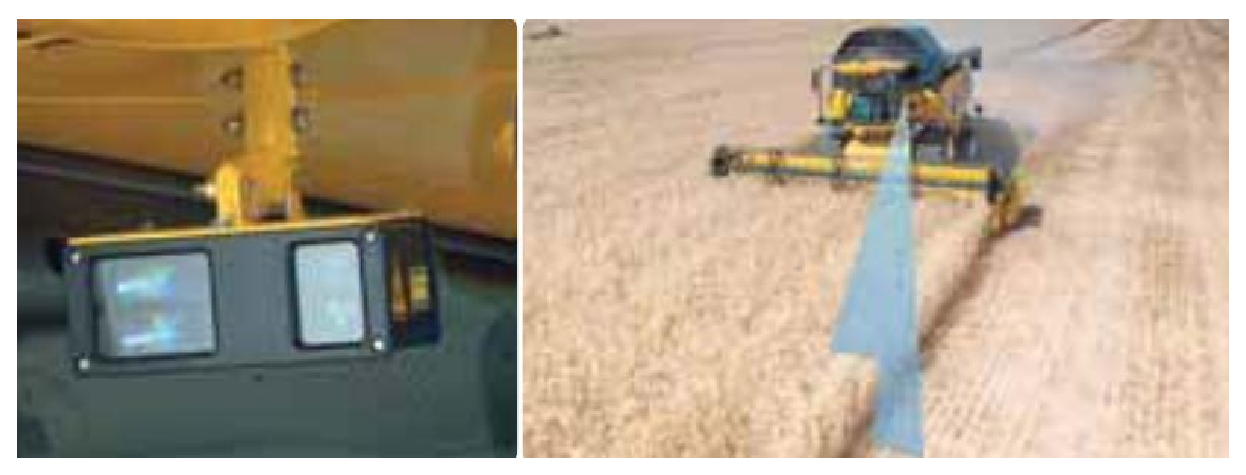
\includegraphics[width=0.7\linewidth]{ch5_new_holland_laser_pilot.eps}
	\caption{System SMARTSTEER firmy New Holland Agriculture}
	\label{fig:new_holland_smartsteer}
\end{figure}
\indent Firma John Deere jako jedyna firma z trzech wybranych do analizy, nie prezentuje rozwiązań opartych o czujniki optyczne w swojej ofercie dotyczącej 
systemów prowadzenia.\\
\indent Podobnie jak w przypadku danych z sensorów INS, tak i dane pochodzące z sensorów wideo nie są jeszcze przetwarzane komercyjnie
za pomocą algorytmów fuzji danych łącznie z danymi nawigacyjnymi GNSS.\\
\indent Na zakończenie tego podrozdziału warto krytycznie spojrzeć na dokładności systemów optycznych w zastosowanich do zbioru plonów.
Jeżeli nawet prawdą jest uzyskanie dokładności 10cm, to na odcinku o długości 100m statystycznie pozostawimy nieomłócony obszar równy 5$m^2$.
Przy załorzeniu szerokości hedera 10m otrzymujemy błąd na poziomie pięciu promili, co daje maksymalnie 40kg na hektar. 
W przypadku pesymistycznym, zakładając błąd prowadzenia rzędu 30cm stracimy około kwintala zborza. 
W realiach polskigo rolnictwa, przy dużym rozdrobnieniu urzytków rolnych lepiej jest stracić nawet dwa kwintale zborza lub 
dać zarobić ten ekwiwalent operatorowi kombajnu niż inwestować w drogie systemy prowadzenia.



\chapter{Perspektywy rozwoju oraz wnioski}
\section{Nadzieje związane z systemem GALILEO}
\section{Dynamiczny rozwój elektronicznych sensorów ruchu}
\section{Wykorzystanie systemu naziemnych stacji referencyjnych ASG-EUPOS}
Dlaczego wciąż potrzebujemy local augmentation systems:
Bo jest duże opóźnienie w dostępie do precyzyjnych produktów IGS takich jak orbity i parametry zegara,
a wyznaczenia rapid są zbyt mało dokładne \cite[][strona 215]{ggos}


%\chapter{Wnioski}
%%\section{Specjalizacja gospodarstw rolnych}
%\section{Wzrost wydajności produkcji}
%\section{Zmniejszenie negatywnego oddziaływania na środowisko}



\appendix
\chapter{Dodatek}
\section{VLBI}
Very Long Baseline Interferometry - Interferometria Długich Baz jest techniką geodezji kosmicznej która powstała w latach 80 ubiegłego wieku.
Polega na obserwacji fali elektromagnetycznej w paśmie częstotliwości radiowych, która jest emitowana przez obiekty pozagalaktyczne (kwazary).\\
\indent Radio-interferometr złorzony z pary anten kierunkowych - radioteleskopów, jak na rysunku \ref{fig:vlbi_antenna}, obserwuje w zadanym przedziale czasu
tylko jedno źródło pozagalaktyczne. W typowej 24 godzinnej sesji obserwacyjnej VLBI uczestniczy zwykle 8 stacji, które obserwują 60 kwazarów kilkukrotnie w ciągu doby.
\cite[][strona 27]{ggos}.
\begin{figure}[H]
\centering
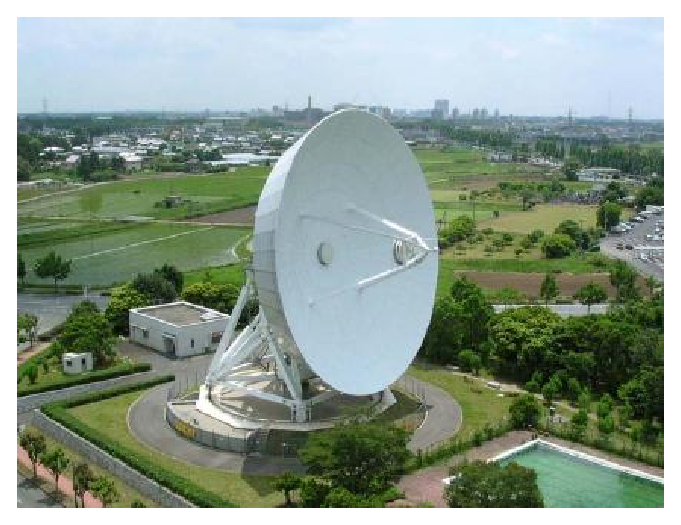
\includegraphics[scale=0.6]{appendix_vlbi_antenna.eps}
\caption{\textit{Antena VLBI o średnicy 32 metrów w mieście Tsukuba, Japonia.} źródło: \cite[][strona 28]{ggos}}
\label{fig:vlbi_antenna}
\end{figure}

\indent Kwazary są tak bardzo oddalone od Układu Słonecznego, że ich ruchy własne są niewykrywalne żadną istniejacą aparaturą. Z punktu widzenia dokładności pomiaru 
uznajemy je zatem za punkty stałe w przestrzeni kosmicznej. Zbiór pozagalaktycznych radio-źródeł realizuje zatem inercjalny układ odniesienia w oparciu o który precyzyjnie
(dokładność rzędu kilku milimetrów) estymowane są pozycje stacji VLBI. Względne prędkości stacji wyznacza się na podstawie kilkuletnich szeregów czasowych obserwacji VLBI 
\cite[][strona 27]{ggos}. Poniżej opisano procedurę wyznaczania współrzędnych wektora o początku i końcu umieszczonych w centrach fazowych radio-interferometru 
\ref{fig:vlbi_principle}.\\
\indent Sygnał radiowy odbierany przez radioteleskop stacji VLBI jest nagrywany cyfrowo z bardzo dokładną referencją czasową dostarczaną przez maser wodorowy. 
\footnote{Maser to urządzenie o zasadzie działania identycznej jak laser, ale emitujące promieniowanie w innym zakresie częstotliwości, która chartakteryzuje się 
wysoką stabilnością. 1s spóźnienia na ponad 10mln lat}
Ten sam sygnał przebywa dodatkową drogę $c\tau$ zanim dotrze do centrum fazowego drugiej anteny interferometru. Gdzie $c$ to prędkość światła, a $\tau$ stanowi 
różnicę czasu dotarcia fali radiowej do obu anten interferometru, wyznaczaną za pomocą korelacji nagranych sygnałów. W ten sposób obliczany jest rzut wektora stanowiącego bazę
na oś w kierunku do badanego radioźródła \cite[][strona 27]{ggos}. 
Na podstawie pomiarów sygnałów pochodzących od różnych radioźródeł, wyznacza się wszystkie współrzędne wektora zdefiniowanego między centrami fazowymi anten 
radiointerferometru w układzie ICRF. 
\begin{figure}[H]
\centering
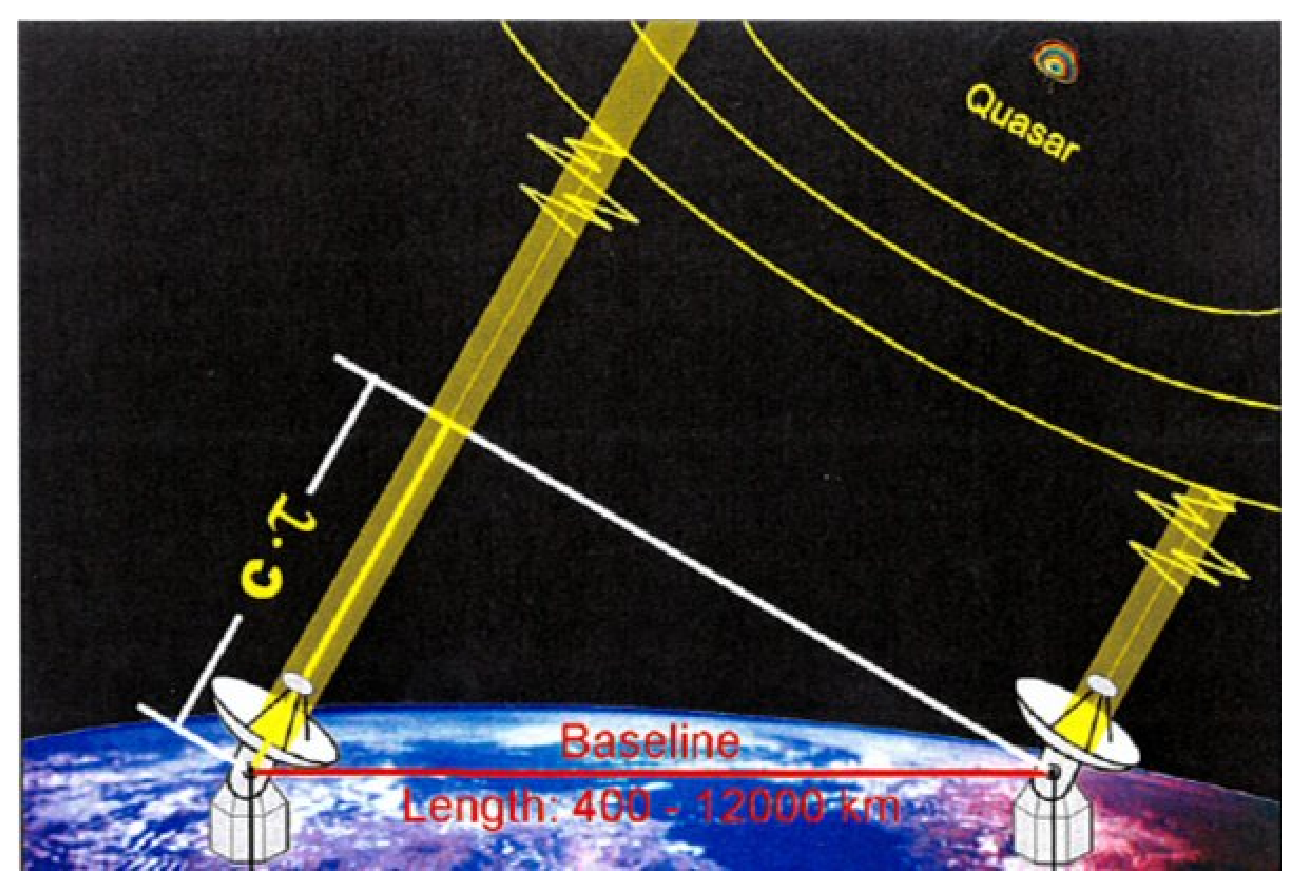
\includegraphics[scale=0.6]{appendix_vlbi_principle.eps}
\caption{\textit{Zasada działania Interferometrii Długich Baz} źródło: \protect\url{http://www.mpifr-bonn.mpg.de/technologie/vlbi}}
\label{fig:vlbi_principle}
\end{figure}



%%%%%%%%%%%%%%%%%%%%%%%%%%%%%%%%%%%%%%%%%%%%%%%%%%%%%%%%%%%%%%%%%%%%%%%%%%%%%%%%%%%%%%%%%%
%			DORIS
%%%%%%%%%%%%%%%%%%%%%%%%%%%%%%%%%%%%%%%%%%%%%%%%%%%%%%%%%%%%%%%%%%%%%%%%%%%%%%%%%%%%%%%%%%
\section{DORIS}
\noindent DORIS (Doppler Orbitography and Radiopositioning Integrated by Satellite) jest francuskim cywilnym systemem montowanym 
na satelitach, służącym głównie do precyzyjnego wyznaczania orbit sztucznych satelitów Ziemi oraz pozycjonowania aktywnych stacji referencyjnych.
Zaprojektowany przez Francuską Agencję Kosmiczną CNES, system bazuje na efekcie Dopplera zmiany częstotliwości fali radiowej rejestrowanej przez odbiornik 
umieszczony na satelicie będącym w ruchu orbitalnym, uzględem częstotliwości referencyjnej sygnału wysłanego ze stacji naziemnej sztywno związanej z Ziemią
 w jej ruchu obrotowym. \cite[]{DORIS_AVISO} System składa się z anteny długości 42 cm, radio-odbiornika oraz wysoko stabilnego generatora częstotliwości wzorcowej. 
Elementy te przedstawia rysunek \ref{fig:DORIS_equipment}.
\begin{figure}[H]
\centering
\begin{subfigure}{.33\textwidth}
  \centering
  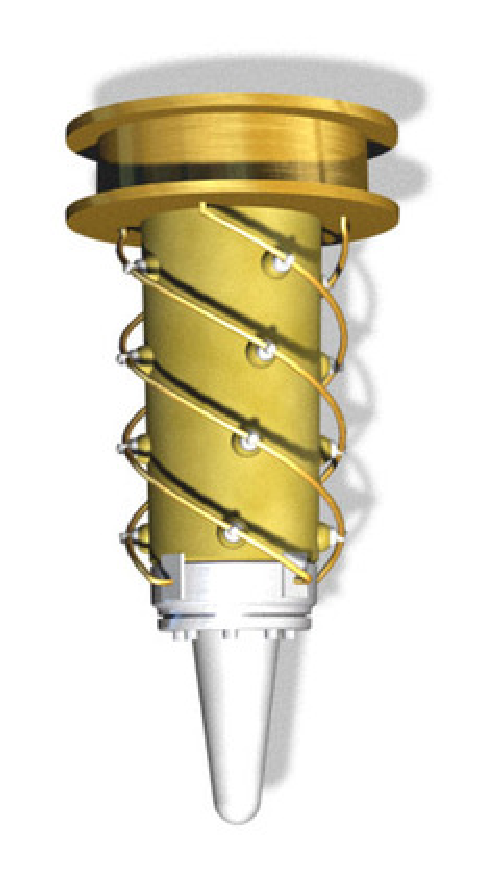
\includegraphics[width=.3\linewidth]{appendix_doris_antenna.eps}
  \caption{antena}
  \label{fig:DORIS_eq_sub1}
\end{subfigure}%
\begin{subfigure}{.3\textwidth}
  \centering
  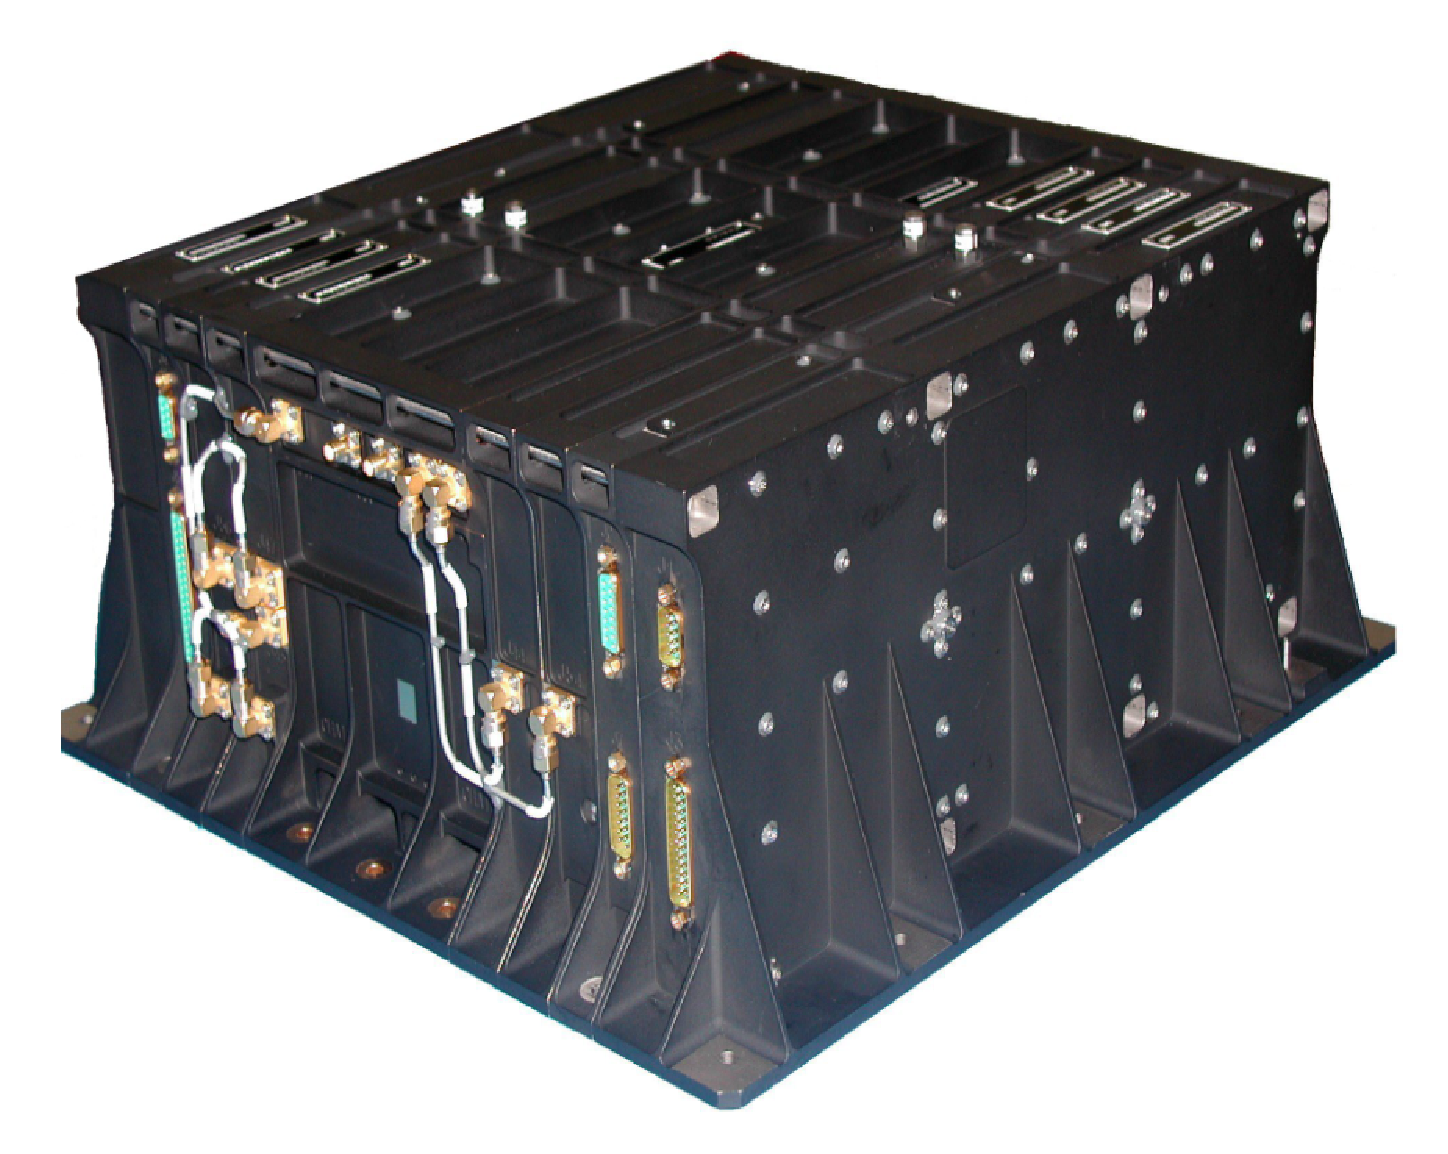
\includegraphics[width=.3\linewidth]{appendix_doris_receiver.eps}
  \caption{odbiornik}
  \label{fig:DORIS_eq_sub2}
\end{subfigure}
\begin{subfigure}{.3\textwidth}
	\centering
	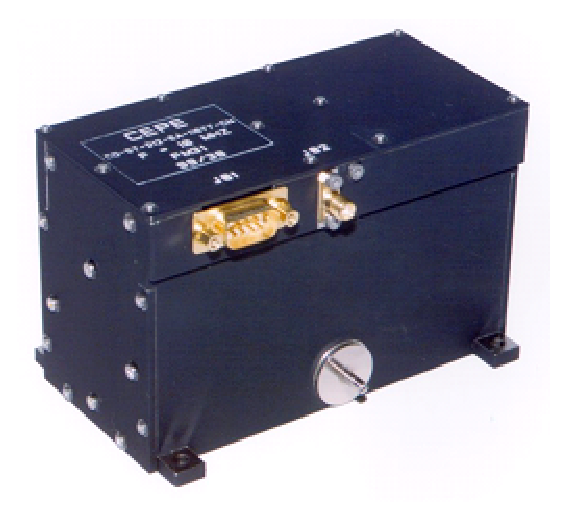
\includegraphics[width=.3\linewidth]{appendix_doris_freequency_generator.eps}
	\caption{generator częstotliwości wzorcowej}
	\label{fig:DORIS_eq_sub3}
\end{subfigure}
\caption{\textit{Komponenty systemu DORIS}
źródło: \protect\url{http://smsc.cnes.fr/DORIS/GP_systeme.htm}}
\label{fig:DORIS_equipment}
\end{figure}

\indent Kiedy satelita z zainstalowanym na pokładzie systemem DORIS zbliża się w kierunku stacji emitującej sygnal referencyjny,
częstotliwość odbieranego przez odbiornik sygnału ulega zwiększeniu. Gdy satelita oddala się od źródła sygnału wtedy odbiornik systemu DORIS 
odbiera sygnał o częstotliwości niższej niż referencyjna. Wykorzystując super stabilny wzorzec częstotliwości referencyjnej system w każdym pomiarze (interwał 10s)
porównuje częstotliwość fali elektromagnetycznej odbieranego sygnału z częstotliwością wzorca. Na podstawie pomiarów dopplerowskiej zmiany częstotliwości,
przy wykorzystaniu filatracji Kalmana oraz algorytmu całkowania numerycznego Runge-Kutta, oprogramowanie o nazwie DIODE wyznacza precyzyjnie 
pozycję oraz prędkość satelity w czasie rzeczywistym \cite[][zakładka: /DORIS system/Diode]{DORIS_AVISO}.\\
\indent Każdy z odbiorników sytemu DORIS przechowuje w pamięci wewnętrznej wszystkie wyniki pomiarów. W momęcie gdy satelita wraz z odbiornikiem 
znajdują się nad stacją referencyjną, wszystkie dane są wysyłane transmisją radiową na ziemię. Obecnie segment naziemny systemu DORIS tworzy około 
60 stacji permanentnych, nieprzerwanie emitujących sygnał referencyjny, równomiernie rozmieszczonych na powierzchni całego Globu.
Wśród stacji permanentnych, których głównym zadaniem jest umożliwianie precyzyjnego wyznaczania orbit, wyróżnić można trzy stacje główne
(Toulouse, Kourou, Harthebeesthoek),
których zadaniem jest synchronizacja czasu systemu z Międzynarodowym Czasem Atomowym (TAI). 
Poniżej na rysunku \ref{fig:doris_infrastructure} zilustrowano sieć stacji referencyjnych opisywanego systemu.
\begin{figure}[H]
\centering
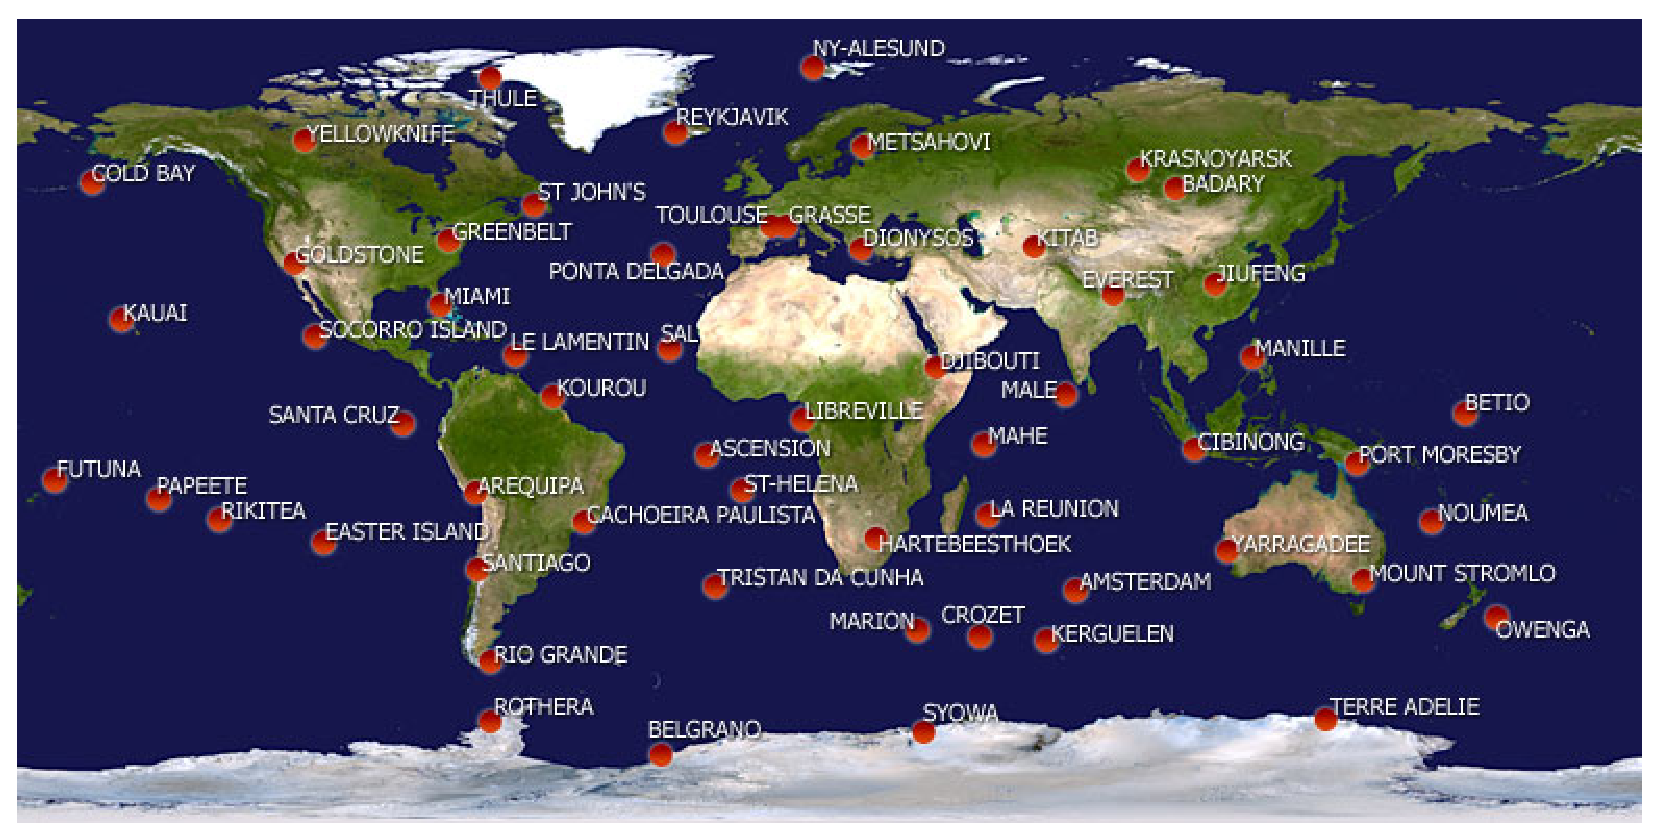
\includegraphics[scale=0.4]{appendix_doris_infrastructure.eps}
\caption{\textit{Mapa aktualnej infrastruktury naziemnej systemu DORIS} źródło: \protect\url{http://ids-doris.org/network/maps.html}}
\label{fig:doris_infrastructure}
\end{figure}
\indent Wszystkie dane zebrane przez stacje segmentu naziemnego są wysyłane do centrum obliczeniowego Ssalto
\footnote{SSALTO multi-mission altimetry, orbit determination and location ground segment (Segment-Sol multi-missions ALTimetrie, Orbitographie et localisation precise)}
w Tuluzie. W centrum obliczeniowym wyznaczane są trajektorie ruchu satelitów wyposarzonych w odbiorniki systemu DORIS. Ssalto jest również odpowiedzialne
za gromadzenie oraz dystrybucję danych pozyskanych za pomocą DORIS
\cite[][zakładka: Control and processing centre]{DORIS_AVISO}.\\
\indent Precyzyjne orbity satelitów wyznaczane za pomocą systemu DORIS znalazły szerokie zastosowanie w altimetrii geodezyjnej (badanie poziomu mórz i oceanów),
na potrzeby badania zmian klimatycznych tak bardzo istotnych dla rolnictwa. 

%%%%%%%%%%%%%%%%%%%%%%%%%%%%%%%%%%%%%%%%%%%%%%%%%%%%%%%%%%%%%%%%%%%%%%%%%%%%%%%%%%%%%%%%%%%%%%%%%
%		SLR
%%%%%%%%%%%%%%%%%%%%%%%%%%%%%%%%%%%%%%%%%%%%%%%%%%%%%%%%%%%%%%%%%%%%%%%%%%%%%%%%%%%%%%%%%%%%%%%%%
\section{SLR}
\noindent SLR (Salellite Laser Ranging)
Pomiary laserowe w których mierzy się odległości 
z stacji referencyjnej do satelitów. Wiązka laserowa odbija się od reflektorów zwrotnych umieszczonych 
na satelicie. Odległość do satelity wyznacza się mierząc czas jaki przebywa fala elektromagnetyczna o 
precyzyjnie określonej częstotliwości do satelity i z powrotem. Na podstawie pomiarów SLR wyznacza się precyzyjnie 
parametry orbit sztucznych satelitów systemów GNSS.\\
\indent Poniżej na podstawie \cite[][zakładka: Stacja Laserowa/informacje ogólne]{BOROWIEC} zaostały wypunktowane najwazniejsze zastosowania obserwacji SLR:
\begin{itemize}
\item wyznaczanie efemeryd sztucznych satelitów Ziemi z centymetrową dokładnością.
\item wyznaczanie zmiennego w czasie położenia geocentrum.
\item monitorowanie parametrów rotacji Ziemi (ruch biegunów i długość doby).
\item wyznaczanie współrzędnych oraz prędkości stacji referencyjnej wykonującej pomiar.
\item wyznaczanie parametrów Międzynarodowego Ziemskiego Układu Odniesienia ITRF oraz jego poprawę.
\end{itemize}
%%%%%%%%%%%%%%%%%%%%%%%%%%%%%%%%%%%%%%%%%%%%%%%%%%%%%%%%%%%%%%%%%%%%%%%%%%%%%%%%%%%%%%
%			LLR
%%%%%%%%%%%%%%%%%%%%%%%%%%%%%%%%%%%%%%%%%%%%%%%%%%%%%%%%%%%%%%%%%%%%%%%%%%%%%%%%%%%%%%
\section{LLR}
\noindent LLR (Lunar Laser Ranging)
Polega na pomiarze laserowym odległości do naturalnego satelity Ziemi - Księżyca.
Kosmonauci z misji Apollo15 umieścili na Księżycu reflektor zwrotny który odbija światło.  
w tym samym kierunku z którego pada źródło. Pomiar odległości wyznacza się wedle tej samej zasady jak w SLR.
Jako ciekawostkę nalezy wspomnieć, że moc lasera jest rzędu kilku gigawatów, a do Ziemi udaje się powrócić 
tylko pojedynczym fotonom.\\
\indent Pomiary te wykorzystywane są w celu wyznaczania chwilowego położenia środka cieżkości naszej planety.
Poniżej na rysunku \ref{fig:LLR_both} są przedstawione pomiary laserowe wykonywane w obserwatorium Greenbelt w USA.
\begin{figure}[H]
\centering
\begin{subfigure}{.5\textwidth}
  \centering
  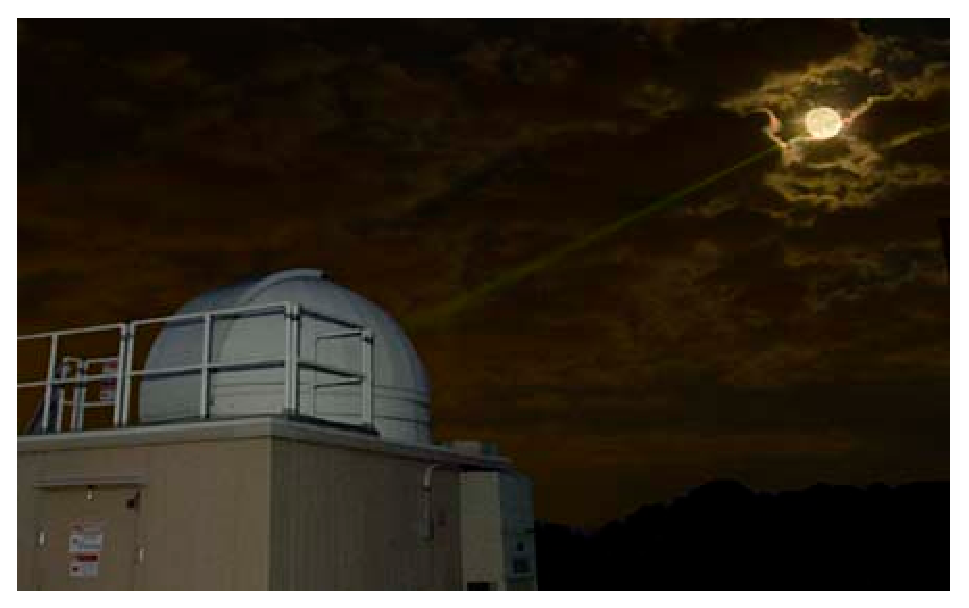
\includegraphics[width=.4\linewidth]{appendix_pomiary_laserowe.eps}
  \caption{}
  \label{fig:LLR_sub1}
\end{subfigure}%
\begin{subfigure}{.5\textwidth}
  \centering
  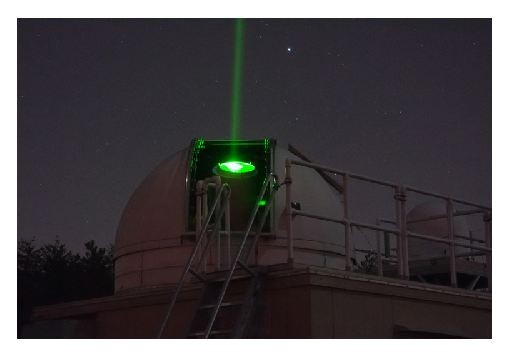
\includegraphics[width=.4\linewidth]{appendix_pomiary_laserowe2.eps}
  \caption{}
  \label{fig:LLR_sub2}
\end{subfigure}
\caption{\textit{Nocne pomiary do księzyca w obserwatorium NASA na stacji GGAO/GSFC w Greenbelt, Maryland, USA}
źródło: \protect\url{http://space-geodesy.gsfc.nasa.gov/multimedia/GeodesyNetwork/GeodesyNetworkImages.html}}
\label{fig:LLR_both}
\end{figure}
%%%%%%%%%%%%%%%%%%%%%%%%%%%%%%%%%%%%%%%%%%%%%%%%%%%%%%%%%%%%%%%%%%%%%%%%%%%%%%%%%%%%%%
% 			POLSKI WKLAD
%%%%%%%%%%%%%%%%%%%%%%%%%%%%%%%%%%%%%%%%%%%%%%%%%%%%%%%%%%%%%%%%%%%%%%%%%%%%%%%%%%%%%

\section{Polski wkład}
\noindent Warto nadmienić, że w Borowcu niedaleko Poznania znajduje się obserwatorium astrogeodynamiczne Centrum Badań Kosmicznych Polskiej Akademii Nauk, 
w którym prowadzone są globalne i lokalne badania geodynamiczne z wykorzystaniem technik GPS oraz SLR.
W ramach obserwatorium działa także grupa Służby Czasu, która partycypuje w tworzeniu międzynarodowej skali czasu atomowego TAI oraz UTC.
Utrzymanie wysokiej dokładności pomiaru czasu (błąd jest obecnie mniejszy niż 2ns) ma kluczowe znaczenie w celu zapewnienia 
wysokiej dokładności pomiarów GNSS. \cite[][zakładka: infomracje ogólne]{BOROWIEC}
\indent W ramach pomiarów SLR stacja badawcza w Borowcu prowadzi pomiary do kilkunastu sztucznych satlitów Zimi. 
W obserwarorium znajduje się także permanentna stacja IGS (jest zaangażowana w dostarczanie najwyższej jakości danych i wyników jako standardu dla Globalnego Systemu Nawigacji Satelitarnej) której odbiorniki zbierają obserwacje z satalitów GPS w sposób ciągły.
Permanentna stacja wchodzi w skład International GNSS service oraz EUREF. W ramach powyższych organizacji definiuje i realizuje Polski oraz Europejski Układ Odniesienia
\cite[][zakładka: Stacja IGS]{BOROWIEC}
 


\listoffigures

\printbibliography[
heading=bibintoc
]
%\bibliographystyle{plain}
%\bibliography{bibliography}


\end{document}
